%% IEEE double-column report (≤ 10 pages)
%% Scalable Cloud Programming CA — MSCCLOUD_JAN26BI
%% Compile: pdflatex ieee_report.tex  (run twice for refs)
\documentclass[conference]{IEEEtran}
\usepackage{cite}
\usepackage{amsmath,amssymb,amsfonts}
\usepackage{graphicx}
\usepackage{textcomp}
\usepackage{xcolor}
\usepackage{booktabs}
\usepackage{url}
\usepackage{hyperref}
\usepackage{float}
\usepackage{multirow}
\usepackage{array}

\graphicspath{{figures/}}

\begin{document}

\title{Scalable Real-Time Wikipedia Event Analytics\\Using Lambda Architecture on AWS}

\author{
\IEEEauthorblockN{Kasireddy Vadicharla}
\IEEEauthorblockA{
\textit{MSc Cloud Computing}\\
Student ID: X25104047\\
National College of Ireland\\
Dublin, Ireland\\
kasireddy9424@gmail.com}
\and
\IEEEauthorblockN{Vishvaksen Machana}
\IEEEauthorblockA{
\textit{MSc Cloud Computing}\\
Student ID: X25173421\\
National College of Ireland\\
Dublin, Ireland\\
mvishvak6768@gmail.com}
}

\maketitle

\begin{abstract}
We design and implement a scalable, cloud-based real-time analytics system on the AWS Academy Learner Lab that ingests the Wikimedia Event Streams recent-change feed, processes events in parallel through a batch layer and a speed layer (Lambda architecture), and serves merged results under elastic compute scaling. Ingestion uses Amazon Kinesis Data Streams with a Python (boto3) producer that dual-writes to Amazon S3 for durable history. The batch layer runs Apache Spark (PySpark) on Amazon EMR to compute accurate full-history aggregates (top Wikipedia projects, keywords, hourly volume). The speed layer applies real-time filtering and a five-minute sliding window to produce low-latency top-$N$ views in DynamoDB, with an optional Spark Structured Streaming path. A serving layer merges Athena (batch parquet) and DynamoDB (speed) results and visualises them via Streamlit on EC2 and CloudWatch. EMR managed scaling (minimum 2, maximum 8 instances) reacts to YARN memory pressure; cooldowns follow EMR managed-scaling defaults. Experiments under high-scale ingest ($>$300\,MB raw object store, order $10^5$ events) demonstrate live throughput, completed EMR batch steps, coherent merge views, and speedup versus worker count. Source code: \url{https://github.com/ScalableCloudProgramming/wikimedia-event-analytics}.
\end{abstract}

\begin{IEEEkeywords}
Lambda architecture, Apache Spark, Amazon Kinesis, EMR, real-time analytics, sliding window, Wikimedia
\end{IEEEkeywords}

\section{Introduction and Objectives}
\subsection{Problem and Real-Time Question}
Wikipedia and sister projects generate a continuous, global stream of edits. Operators, researchers, and community tools need both \emph{immediate} visibility into which projects are hot \emph{right now} and \emph{correct} long-horizon rankings over all data observed so far. Batch-only pipelines deliver correctness but lag the live stream; stream-only pipelines deliver freshness but struggle to recompute accurate full-history views cheaply and consistently after late data, reprocessing, or schema drift.

\textbf{Real-time question answered by this system:}
\begin{quote}
\textit{Which Wikipedia projects receive the most edits in the last 5 minutes (speed), over the full accumulated history (batch), and in a single merged ranking (serving layer)?}
\end{quote}
Secondary aggregates include keyword frequency from page titles and hourly edit volume for capacity planning.

\subsection{Why Lambda Architecture (Batch + Speed)}
A Lambda architecture is appropriate rather than batch-only or stream-only for three reasons:
\begin{enumerate}
\item \textbf{Correctness:} The batch layer recomputes comprehensive views over all raw events on S3 with Spark, so rankings remain accurate as history grows.
\item \textbf{Freshness:} The speed layer maintains incremental, windowed counts with low latency so the last five minutes remain visible without waiting for the next batch job.
\item \textbf{Query simplicity:} The serving layer answers the product question by merging batch totals with the recent speed delta, instead of forcing clients to understand two stores.
\end{enumerate}
Batch-only would miss short-lived spikes between jobs; stream-only would not efficiently recompute full-history top-$N$ with the same guarantees as a Spark job over the complete raw archive.

\subsection{Objectives}
\begin{itemize}
\item Ingest a continuous public stream into AWS (Kinesis) with Python.
\item Process in parallel: Spark batch (full history) and windowed speed layer (recent data).
\item Store and visualise results with AWS services (S3, DynamoDB, Athena, CloudWatch) and a Streamlit dashboard on EC2.
\item Auto-scale EMR compute with stated triggers and cooldowns.
\item Measure throughput, latency behaviour under load, and batch speedup; report critically.
\end{itemize}

\section{Architecture, Tools, and AWS Setup}
\subsection{Architecture Overview}
Figure~\ref{fig:arch} summarises the pipeline. Continuous Wikimedia Server-Sent Events (SSE) enter a Python producer. Each record is published to Kinesis (speed path) and buffered to S3 as JSONL (batch path). The speed consumer updates a time-bucketed sliding window and writes top-$N$ ranks to DynamoDB. Periodically, EMR runs a PySpark job over all raw objects and writes parquet aggregates to S3, registered for Athena. The serving layer merges Athena batch rows with DynamoDB speed rows. Streamlit on EC2 visualises metrics and merge results. The dashed box is the auto-scaling compute boundary (EMR managed scaling for Spark workers; fixed EC2 roles for producer, speed consumer, and dashboard).

\begin{figure}[t]
\centering
\fbox{\parbox{0.95\columnwidth}{\centering\small
\textbf{Lambda Architecture --- Wikimedia Event Analytics}\\[4pt]
\begin{tabular}{@{}c@{}}
Wikimedia SSE stream\\
$\downarrow$\\
\textbf{Ingestion (EC2):} Python producer $\rightarrow$ Kinesis + S3 raw JSONL\\
$\swarrow\qquad\qquad\searrow$\\
\begin{tabular}{@{}c@{\quad}c@{}}
\textbf{Speed layer (EC2)} & \textbf{Batch layer (EMR Spark)}\\
filter + 5-min sliding window & full-history aggregates\\
$\rightarrow$ DynamoDB top-$N$ & $\rightarrow$ S3 parquet $\rightarrow$ Athena\\
\end{tabular}\\
$\searrow\qquad\qquad\swarrow$\\
\textbf{Serving:} merge batch + speed; Streamlit + CloudWatch\\
\textit{Auto-scaling boundary: EMR managed scaling (YARN pressure)}
\end{tabular}}}
\caption{Lambda architecture: ingestion, parallel batch/speed paths, serving merge, and auto-scaling boundary.}
\label{fig:arch}
\end{figure}

\begin{figure}[t]
\centering
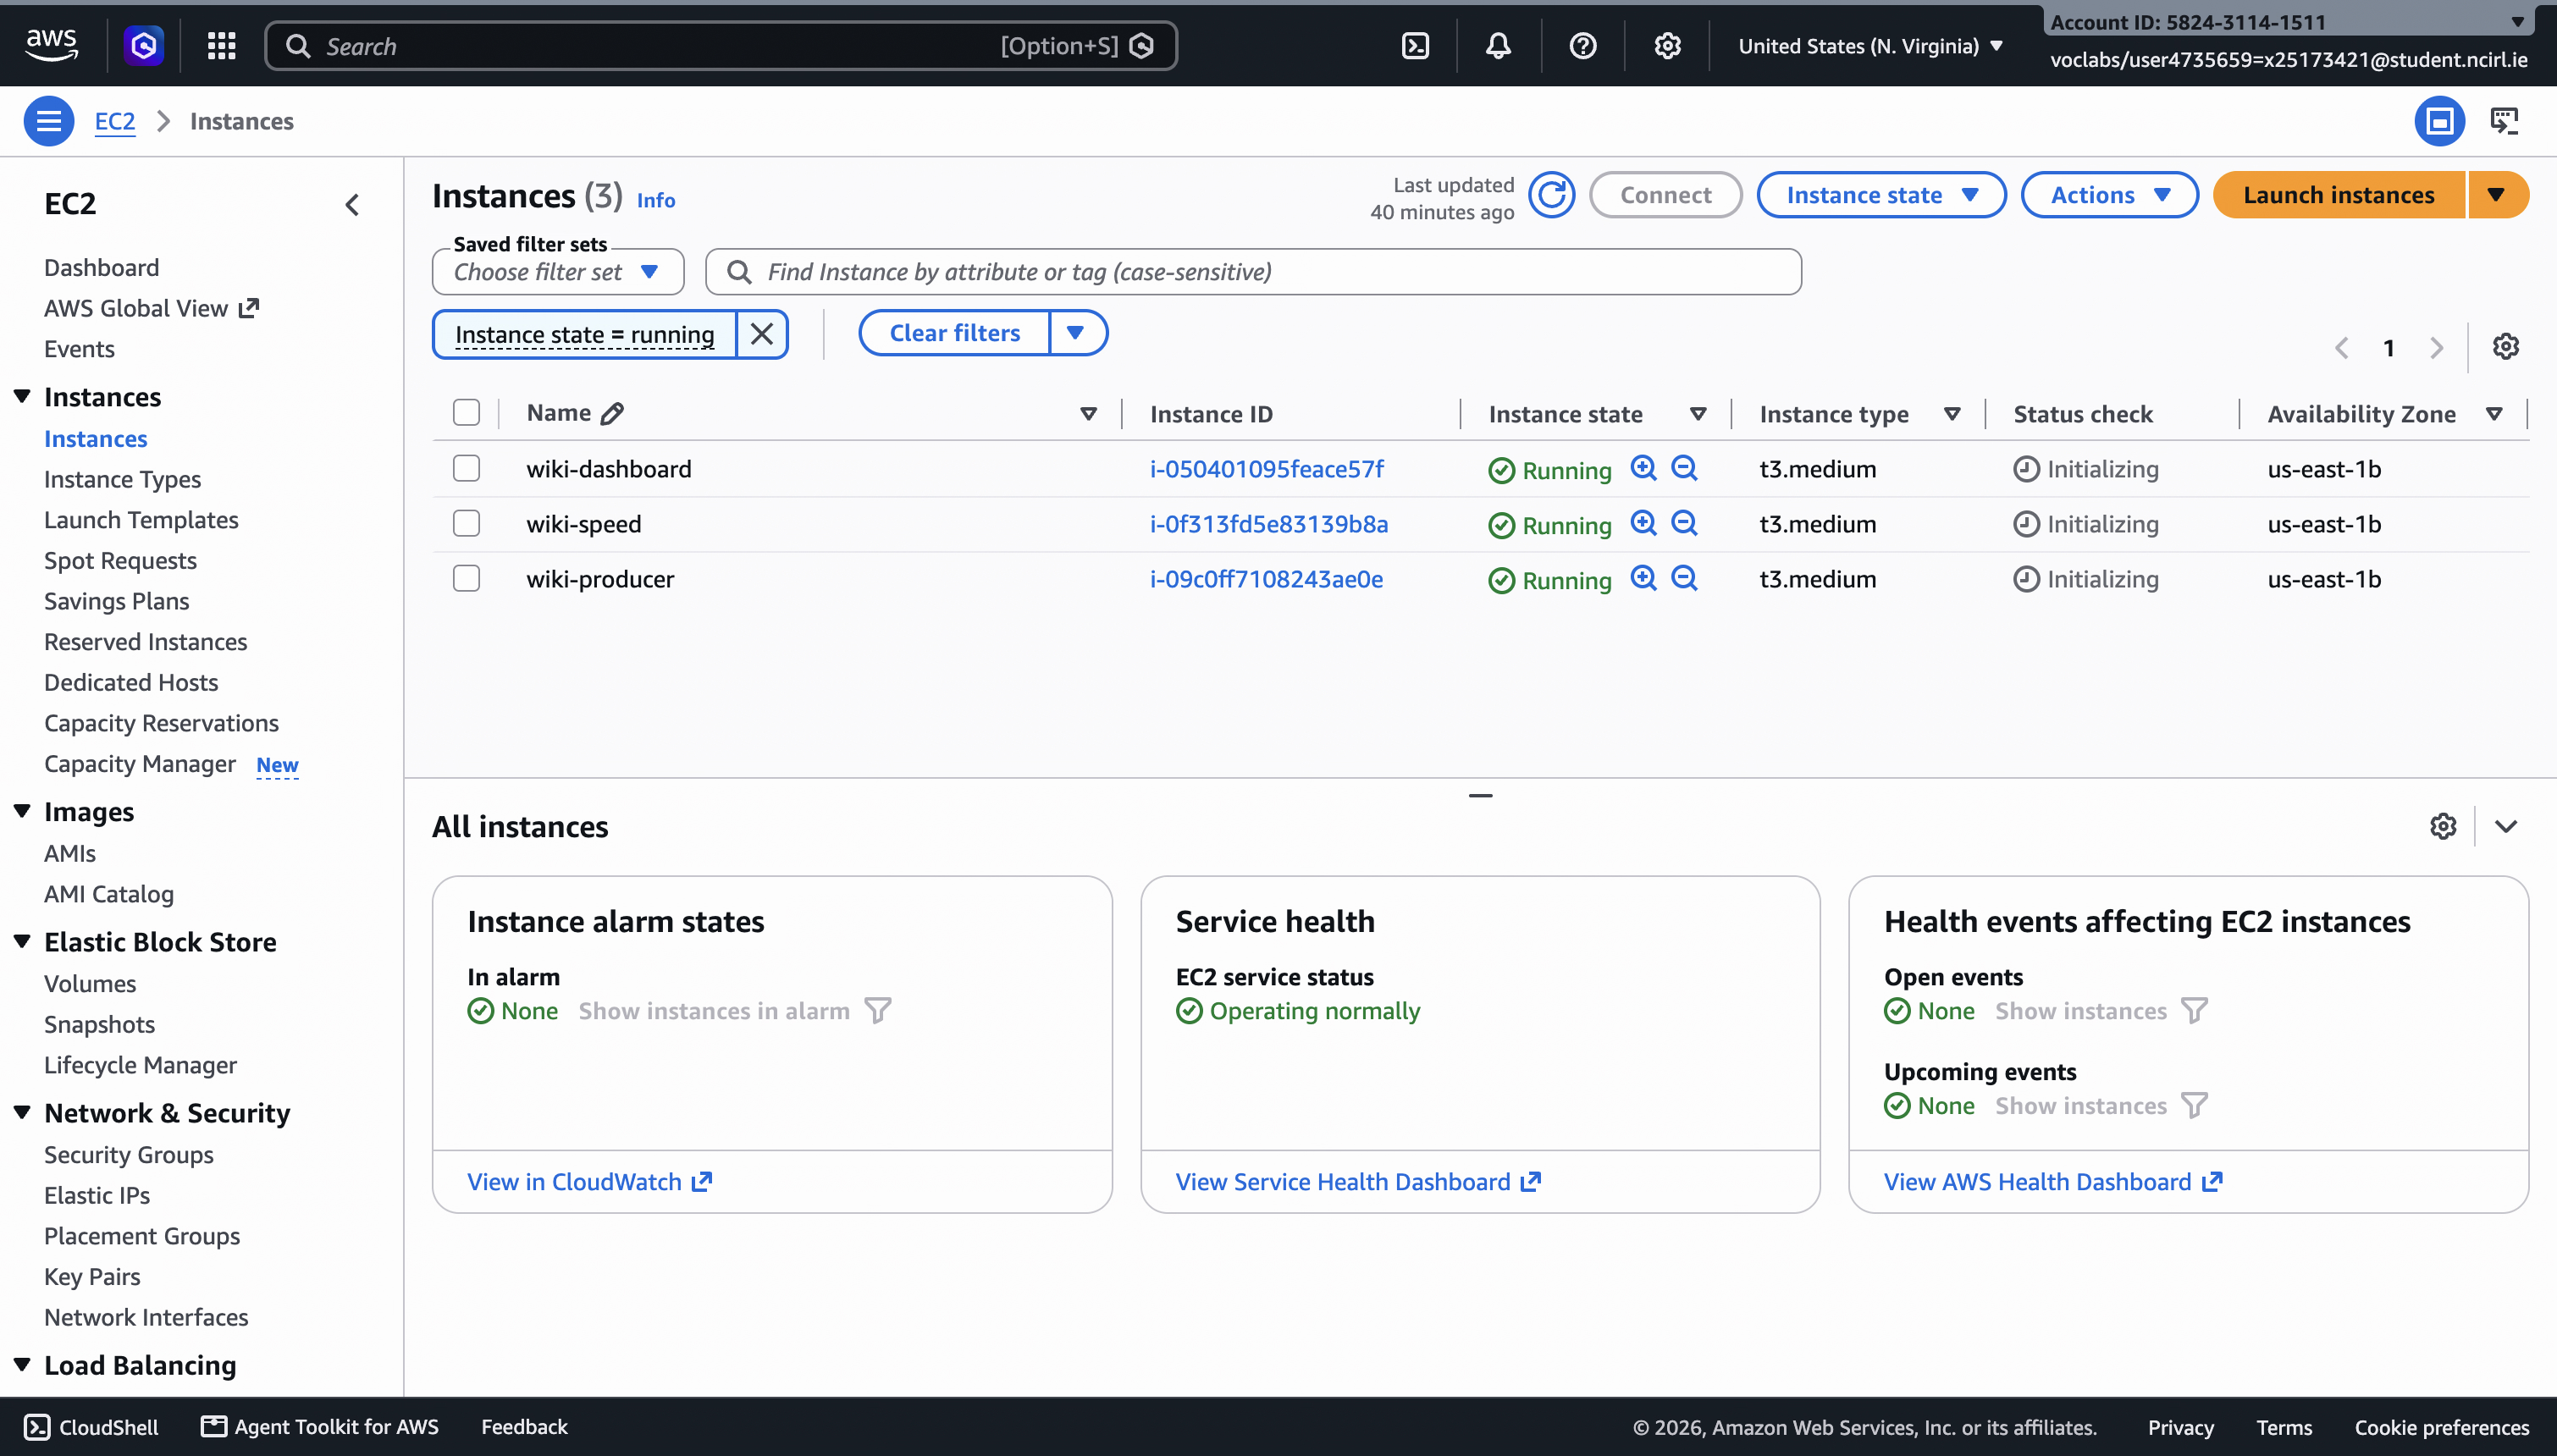
\includegraphics[width=\columnwidth]{01_ec2_fleet.png}
\caption{AWS Academy EC2 fleet: high-scale producer, speed consumer, and Streamlit dashboard instances (running).}
\label{fig:ec2}
\end{figure}

\subsection{Tools and AWS Services}
\begin{table}[t]
\centering
\caption{Primary tools and AWS services}
\label{tab:tools}
\small
\begin{tabular}{@{}ll@{}}
\toprule
\textbf{Layer} & \textbf{Technology} \\
\midrule
Language & Python 3, boto3, requests, sseclient \\
Ingestion & Amazon Kinesis Data Streams (4 shards) \\
Raw store & Amazon S3 (JSONL partitions by time) \\
Batch & Apache Spark 3.x / PySpark on Amazon EMR 6.15 \\
Speed & Custom sliding window; DynamoDB on-demand \\
Speed (alt.) & Spark Structured Streaming (windowed) \\
Serving & Amazon Athena + DynamoDB merge \\
Visualisation & Streamlit on EC2; CloudWatch dashboards \\
Scale & EMR managed scaling; CloudWatch alarms \\
\bottomrule
\end{tabular}
\end{table}

Deployment used the AWS Academy Learner Lab (region \texttt{us-east-1}), IAM instance profile \texttt{LabInstanceProfile}, and shared project resource names (\texttt{wikimedia-stream}, \texttt{wikimedia-analytics-raw/batch}, \texttt{wikimedia-speed-view}).

\subsection{Auto-Scaling: Triggers and Cooldowns}
We configure \textbf{EMR managed scaling} on the batch cluster:
\begin{itemize}
\item \textbf{Unit:} instances (core/task capacity).
\item \textbf{Minimum / maximum:} 2 / 8 instances (environment-configurable).
\item \textbf{Scaling trigger:} YARN resource (memory) pressure under managed scaling---when remaining capacity is insufficient for pending Spark tasks, EMR adds capacity within the max bound.
\item \textbf{Cooldown-down:} when pressure abates, EMR removes capacity subject to \textbf{EMR managed-scaling default cooldown} behaviour (sustained metrics, not instantaneous flapping).
\item \textbf{Observability:} CloudWatch alarms on Kinesis \texttt{IncomingRecords} (high ingest) and \texttt{GetRecords.IteratorAgeMilliseconds} (consumer lag) support operational scaling decisions and demos.
\end{itemize}
Producer, speed consumer, and dashboard run on dedicated EC2 instances sized for continuous load; EMR absorbs elastic batch parallelism.

\section{Implementation}
\subsection{Data Ingestion}
The producer connects to
\texttt{https://stream.wikimedia.org/v2/stream/recentchange}
with a descriptive User-Agent, parses SSE JSON, and calls Kinesis \texttt{put\_record}/\texttt{put\_records}. A buffered \textbf{S3 raw sink} flushes JSONL objects under \texttt{data/yyyy/mm/dd/HH/} so the batch layer always has a complete durable history. High-scale mode multiplies live events (fan-out) and adds controlled synthetic domain-like traffic to stress shards and the speed layer while remaining representative of wiki edit payloads. USGS and local JSONL replay modes are also supported for offline testing.

\begin{figure}[t]
\centering
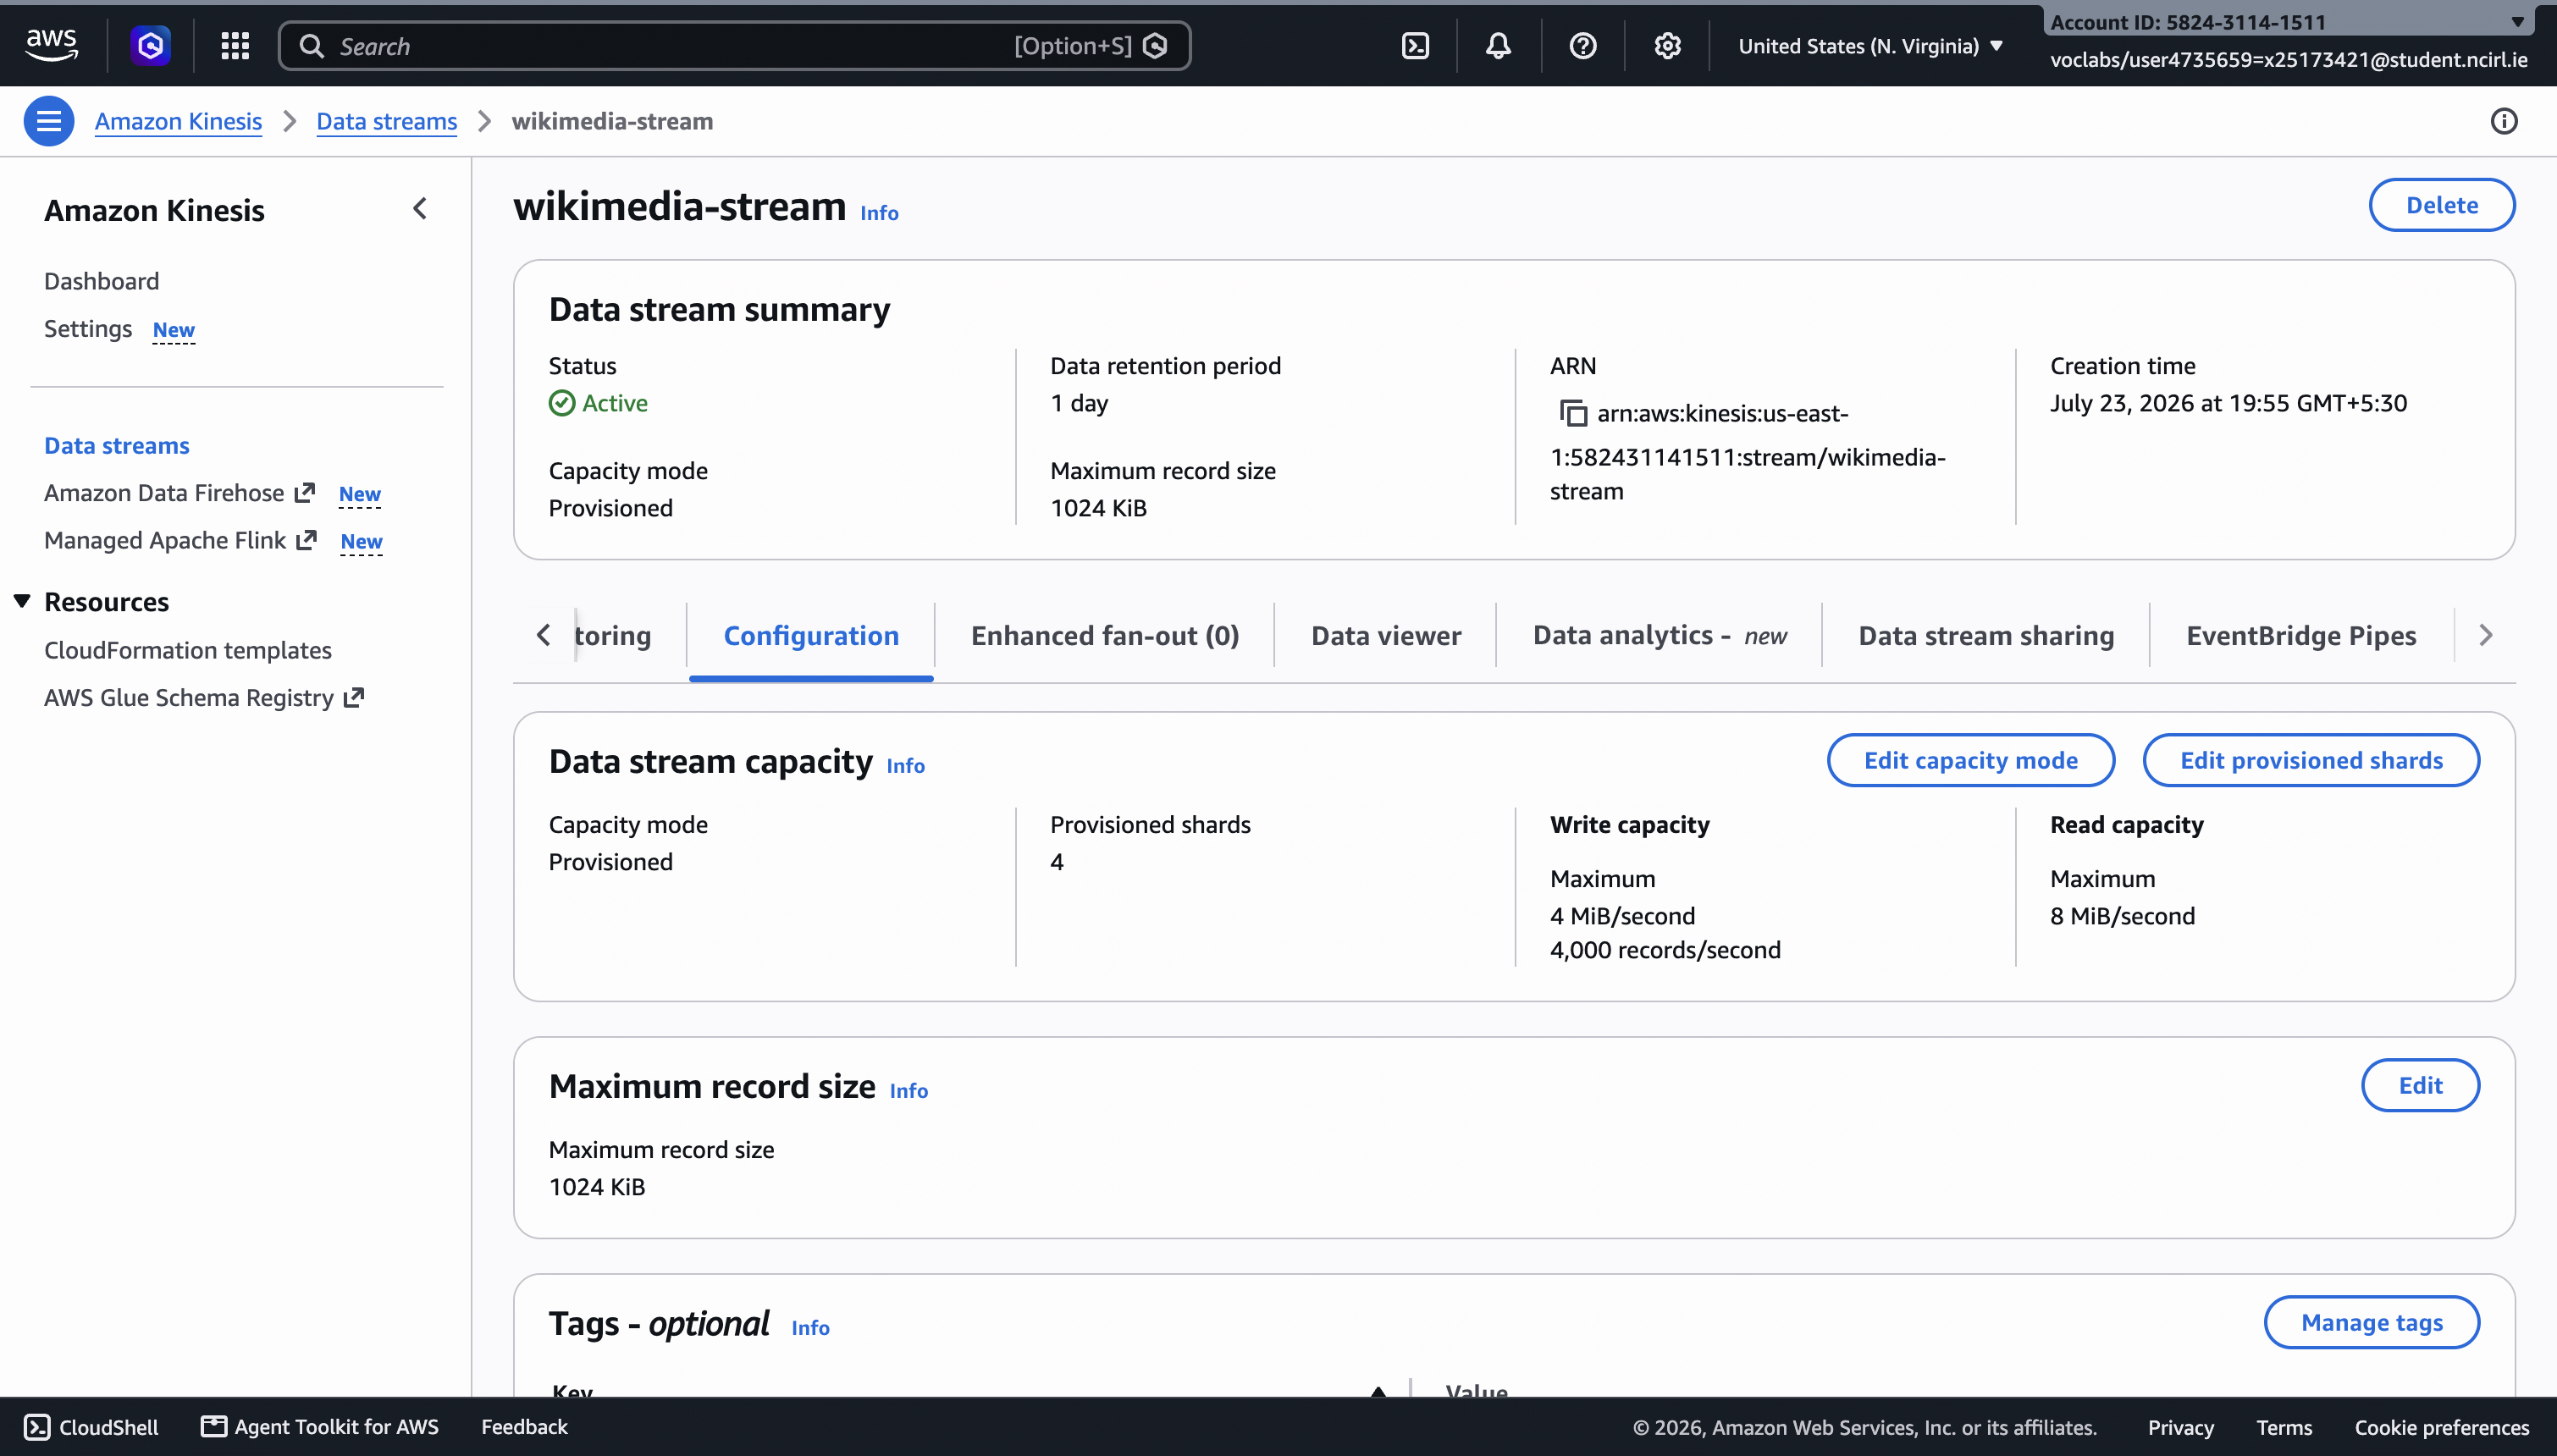
\includegraphics[width=\columnwidth]{02_kinesis_stream.png}
\caption{Kinesis stream \texttt{wikimedia-stream} active with four provisioned shards.}
\label{fig:kinesis}
\end{figure}

\begin{figure}[t]
\centering
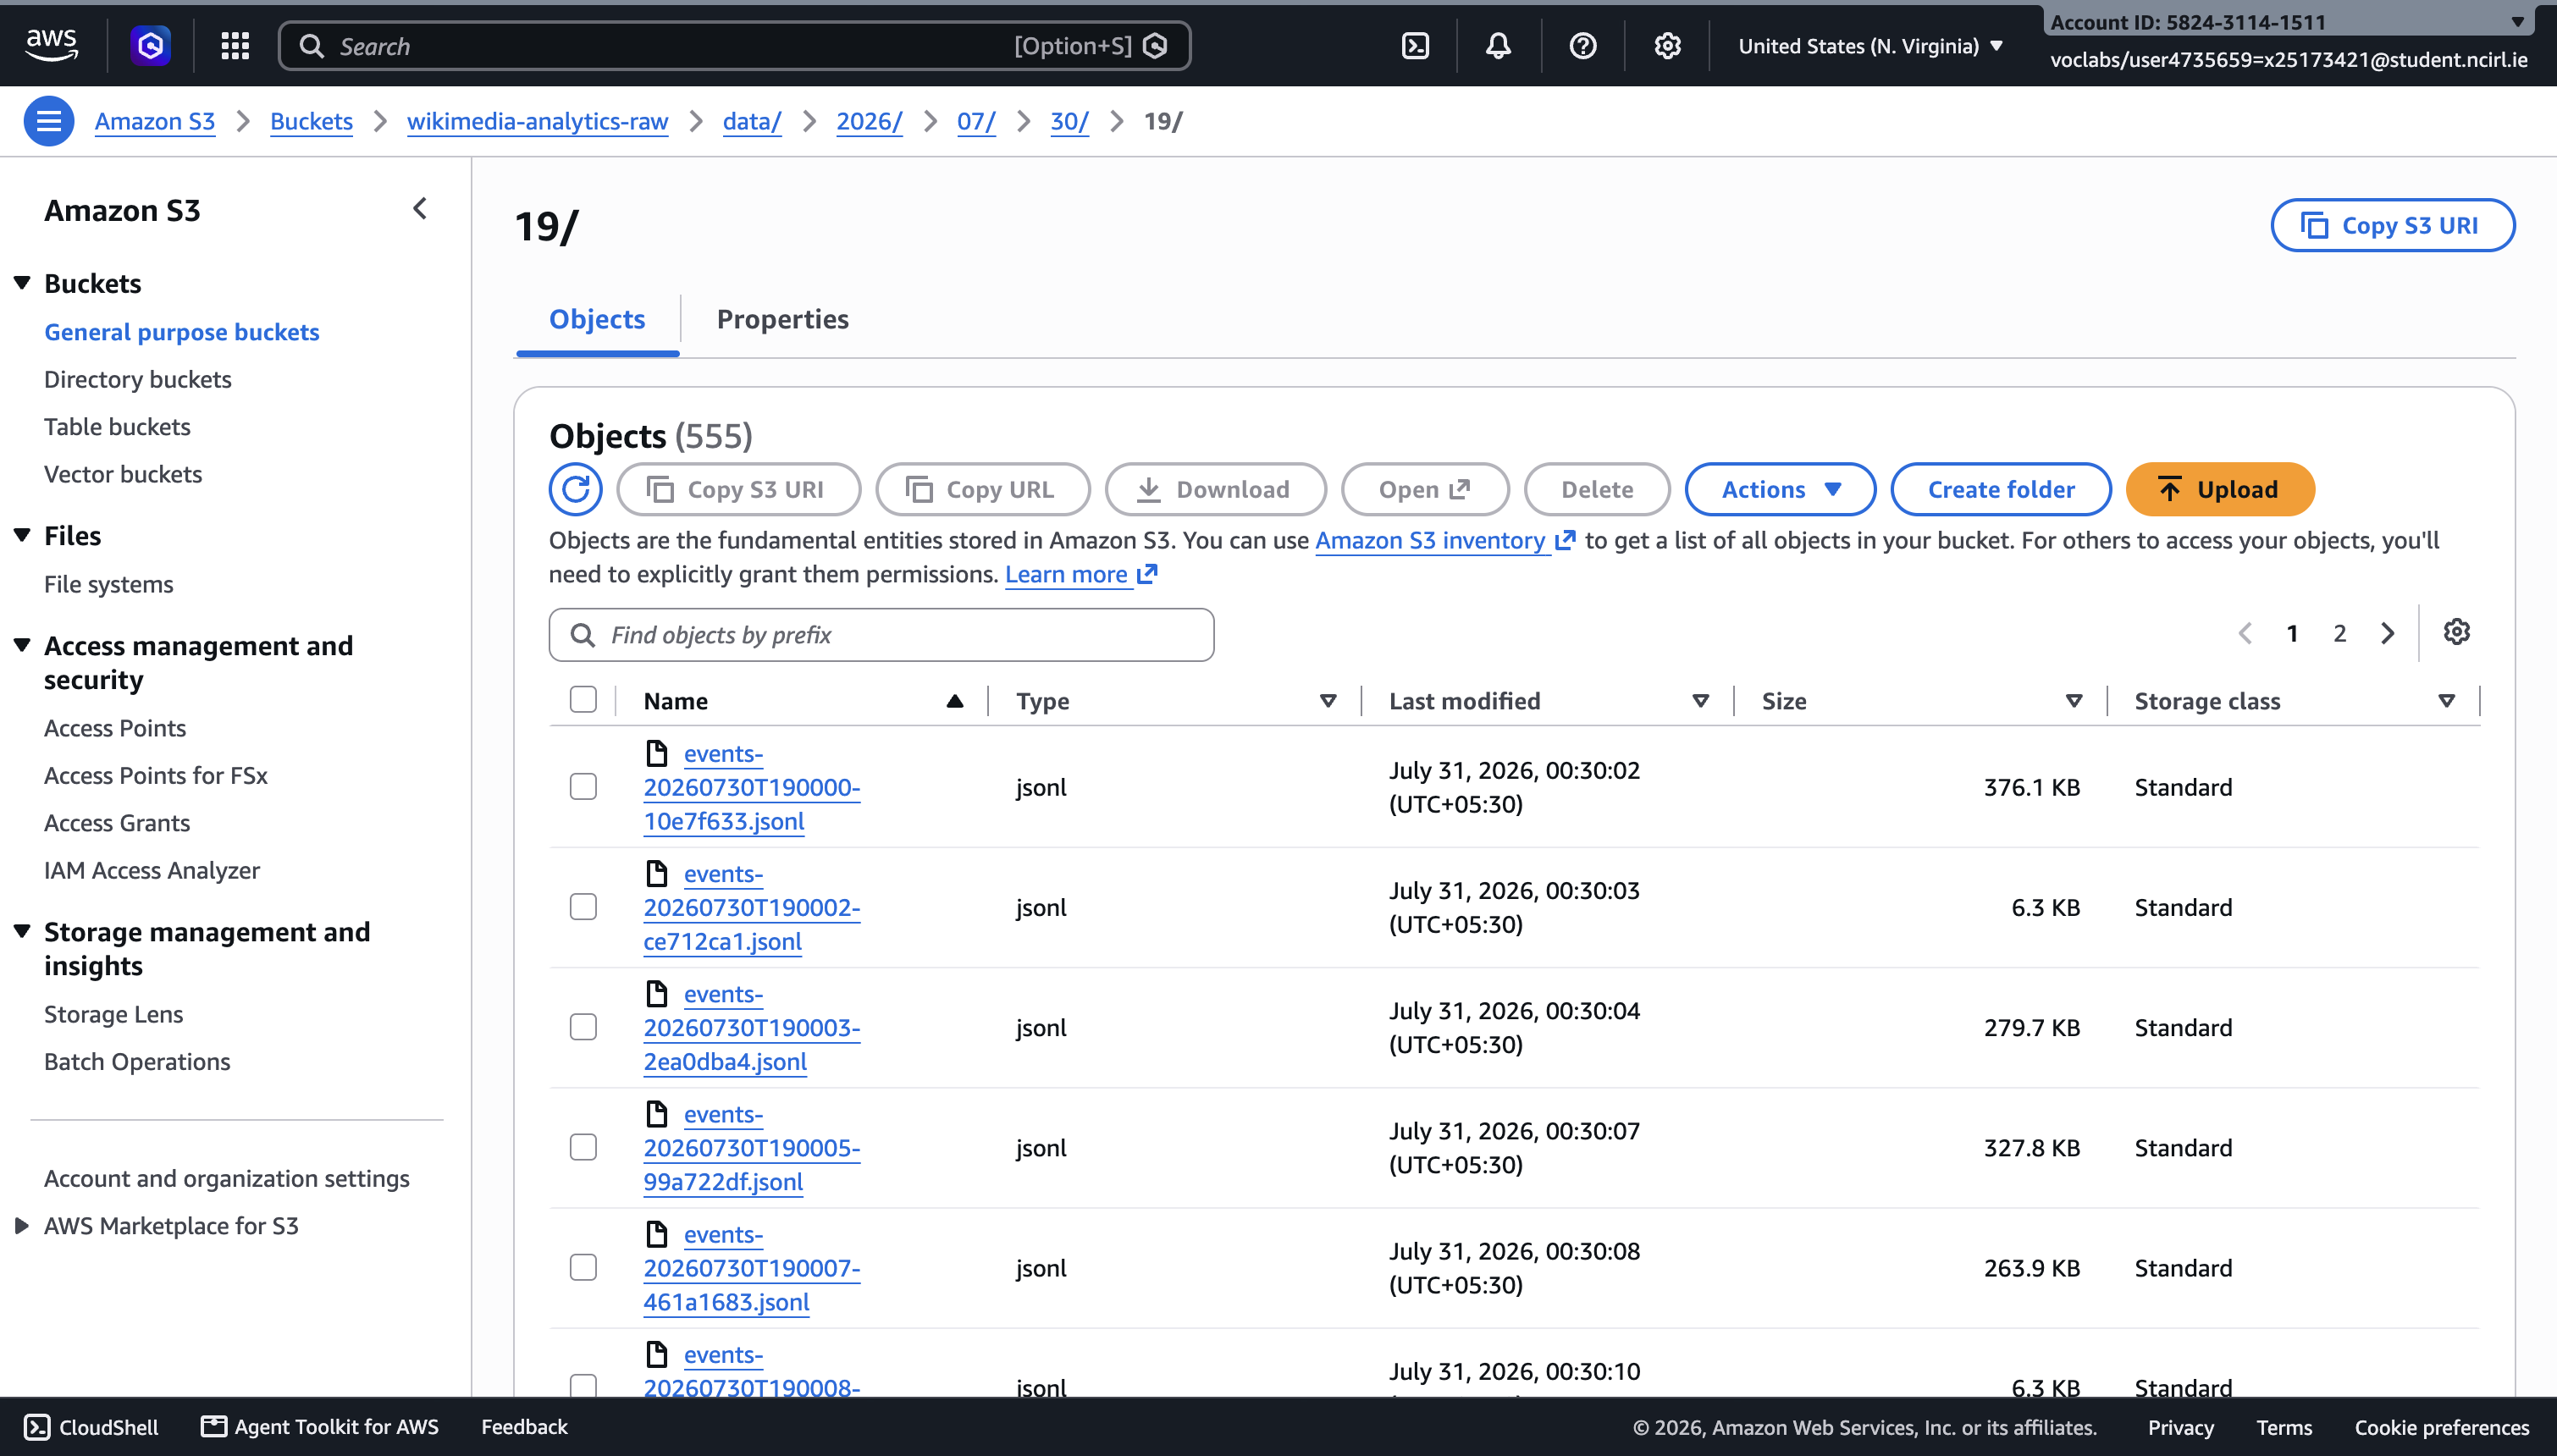
\includegraphics[width=\columnwidth]{05_s3_raw_volume.png}
\caption{Raw ingest on S3: large numbers of JSONL objects under time-partitioned prefixes (scaled run).}
\label{fig:s3raw}
\end{figure}

\subsection{Batch Layer (Spark on EMR)}
The batch job reads all recursive JSONL under the raw prefix with an explicit schema (required because heterogeneous fan-out records break Spark auto-inference), optionally filters bot edits, and writes parquet:
\begin{itemize}
\item Top-$N$ projects by edit count (\texttt{wiki\_edits});
\item Keyword frequencies from titles;
\item Hourly volumes;
\item Edit-type and namespace breakdowns.
\end{itemize}
Jobs are uploaded to S3 and submitted with \texttt{spark-submit} on YARN (cluster/client modes tested). A completed step on EMR produced accurate Athena-queryable tables (e.g., \texttt{commonswiki} $\approx 53{,}009$ full-history edits in the evaluated snapshot). Data parallelism arises from Spark partitions; task parallelism from multi-executor EMR workers.

\begin{figure}[t]
\centering
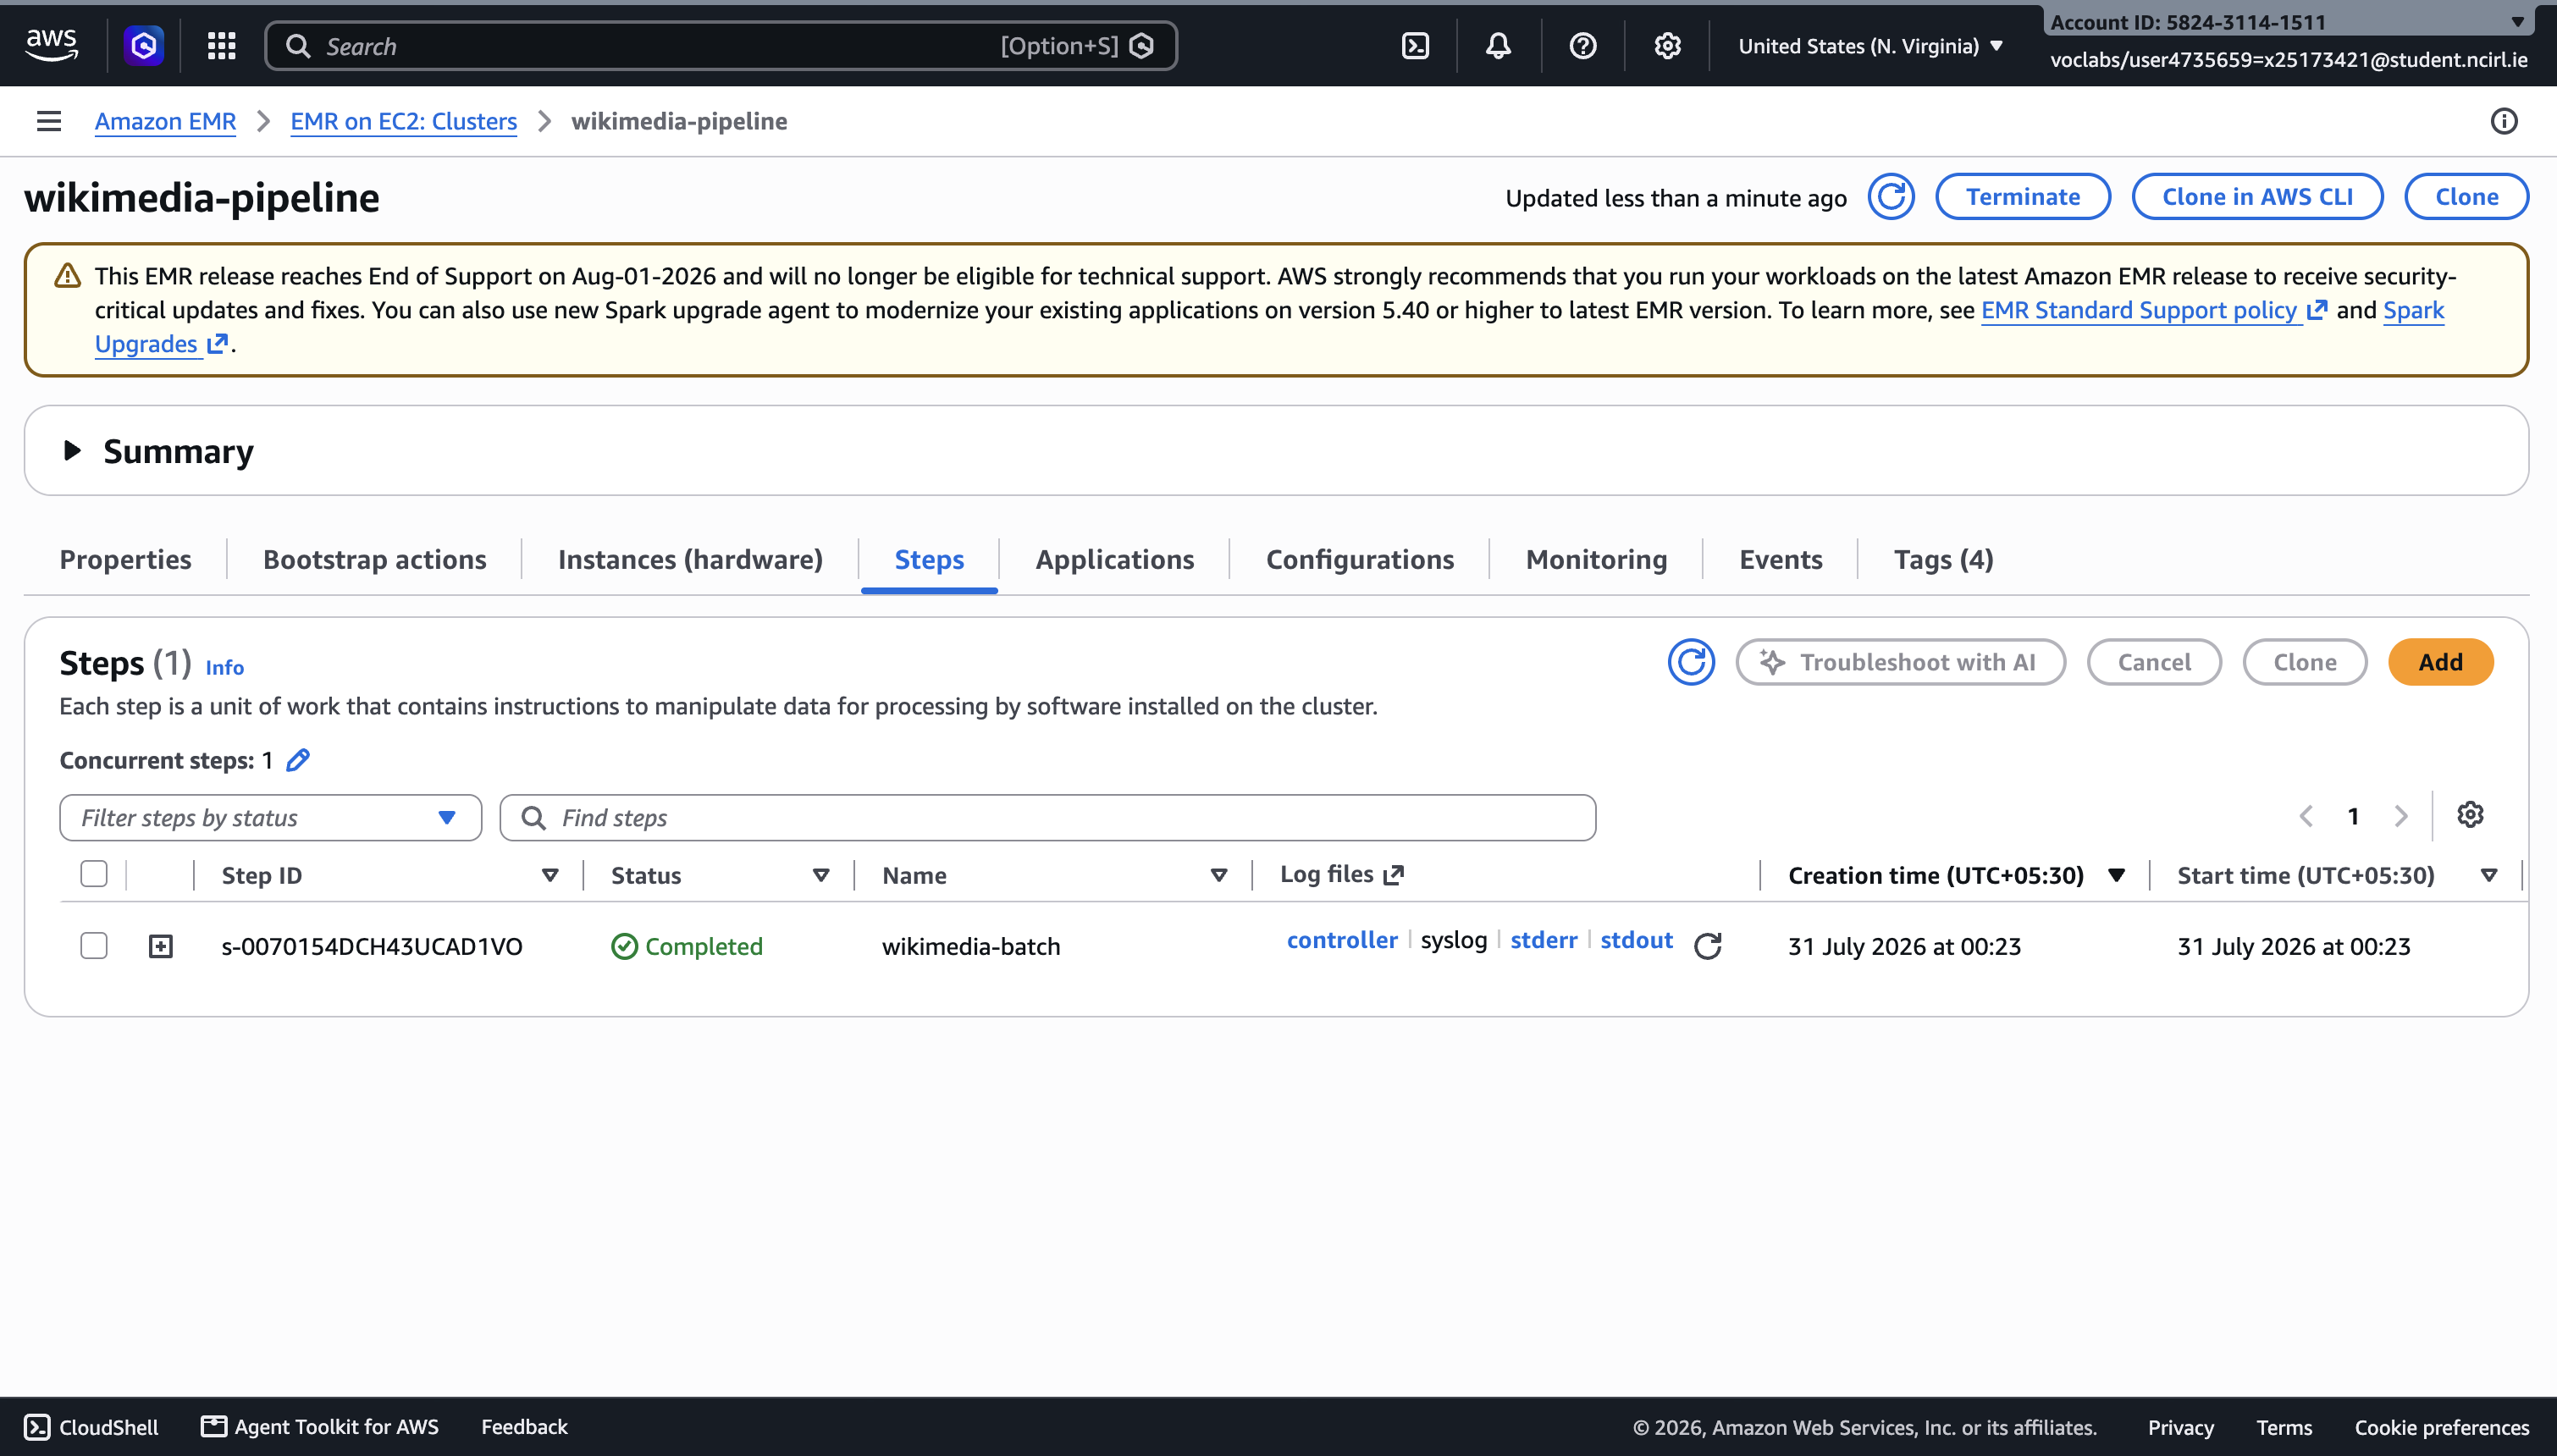
\includegraphics[width=\columnwidth]{09_emr_step_completed.png}
\caption{EMR step \texttt{wikimedia-batch} completed successfully.}
\label{fig:emrstep}
\end{figure}

\subsection{Speed Layer (Sliding Window)}
The speed consumer reads all Kinesis shards, filters bots and non-content event types when fields exist, and updates a \textbf{time-bucketed sliding window} (default window $W=300$\,s, bucket $10$\,s). Buckets older than $W$ are evicted. Top-$N$ wikis are flushed to DynamoDB keys \texttt{speed\#1..N}, enabling continuous incremental views. This realises the brief's distinction criterion: top projects in the last $N$ minutes. Spark Structured Streaming provides an alternative path with \texttt{window(event\_time, 5 minutes, 1 minute)} to S3 parquet.

\begin{figure}[t]
\centering
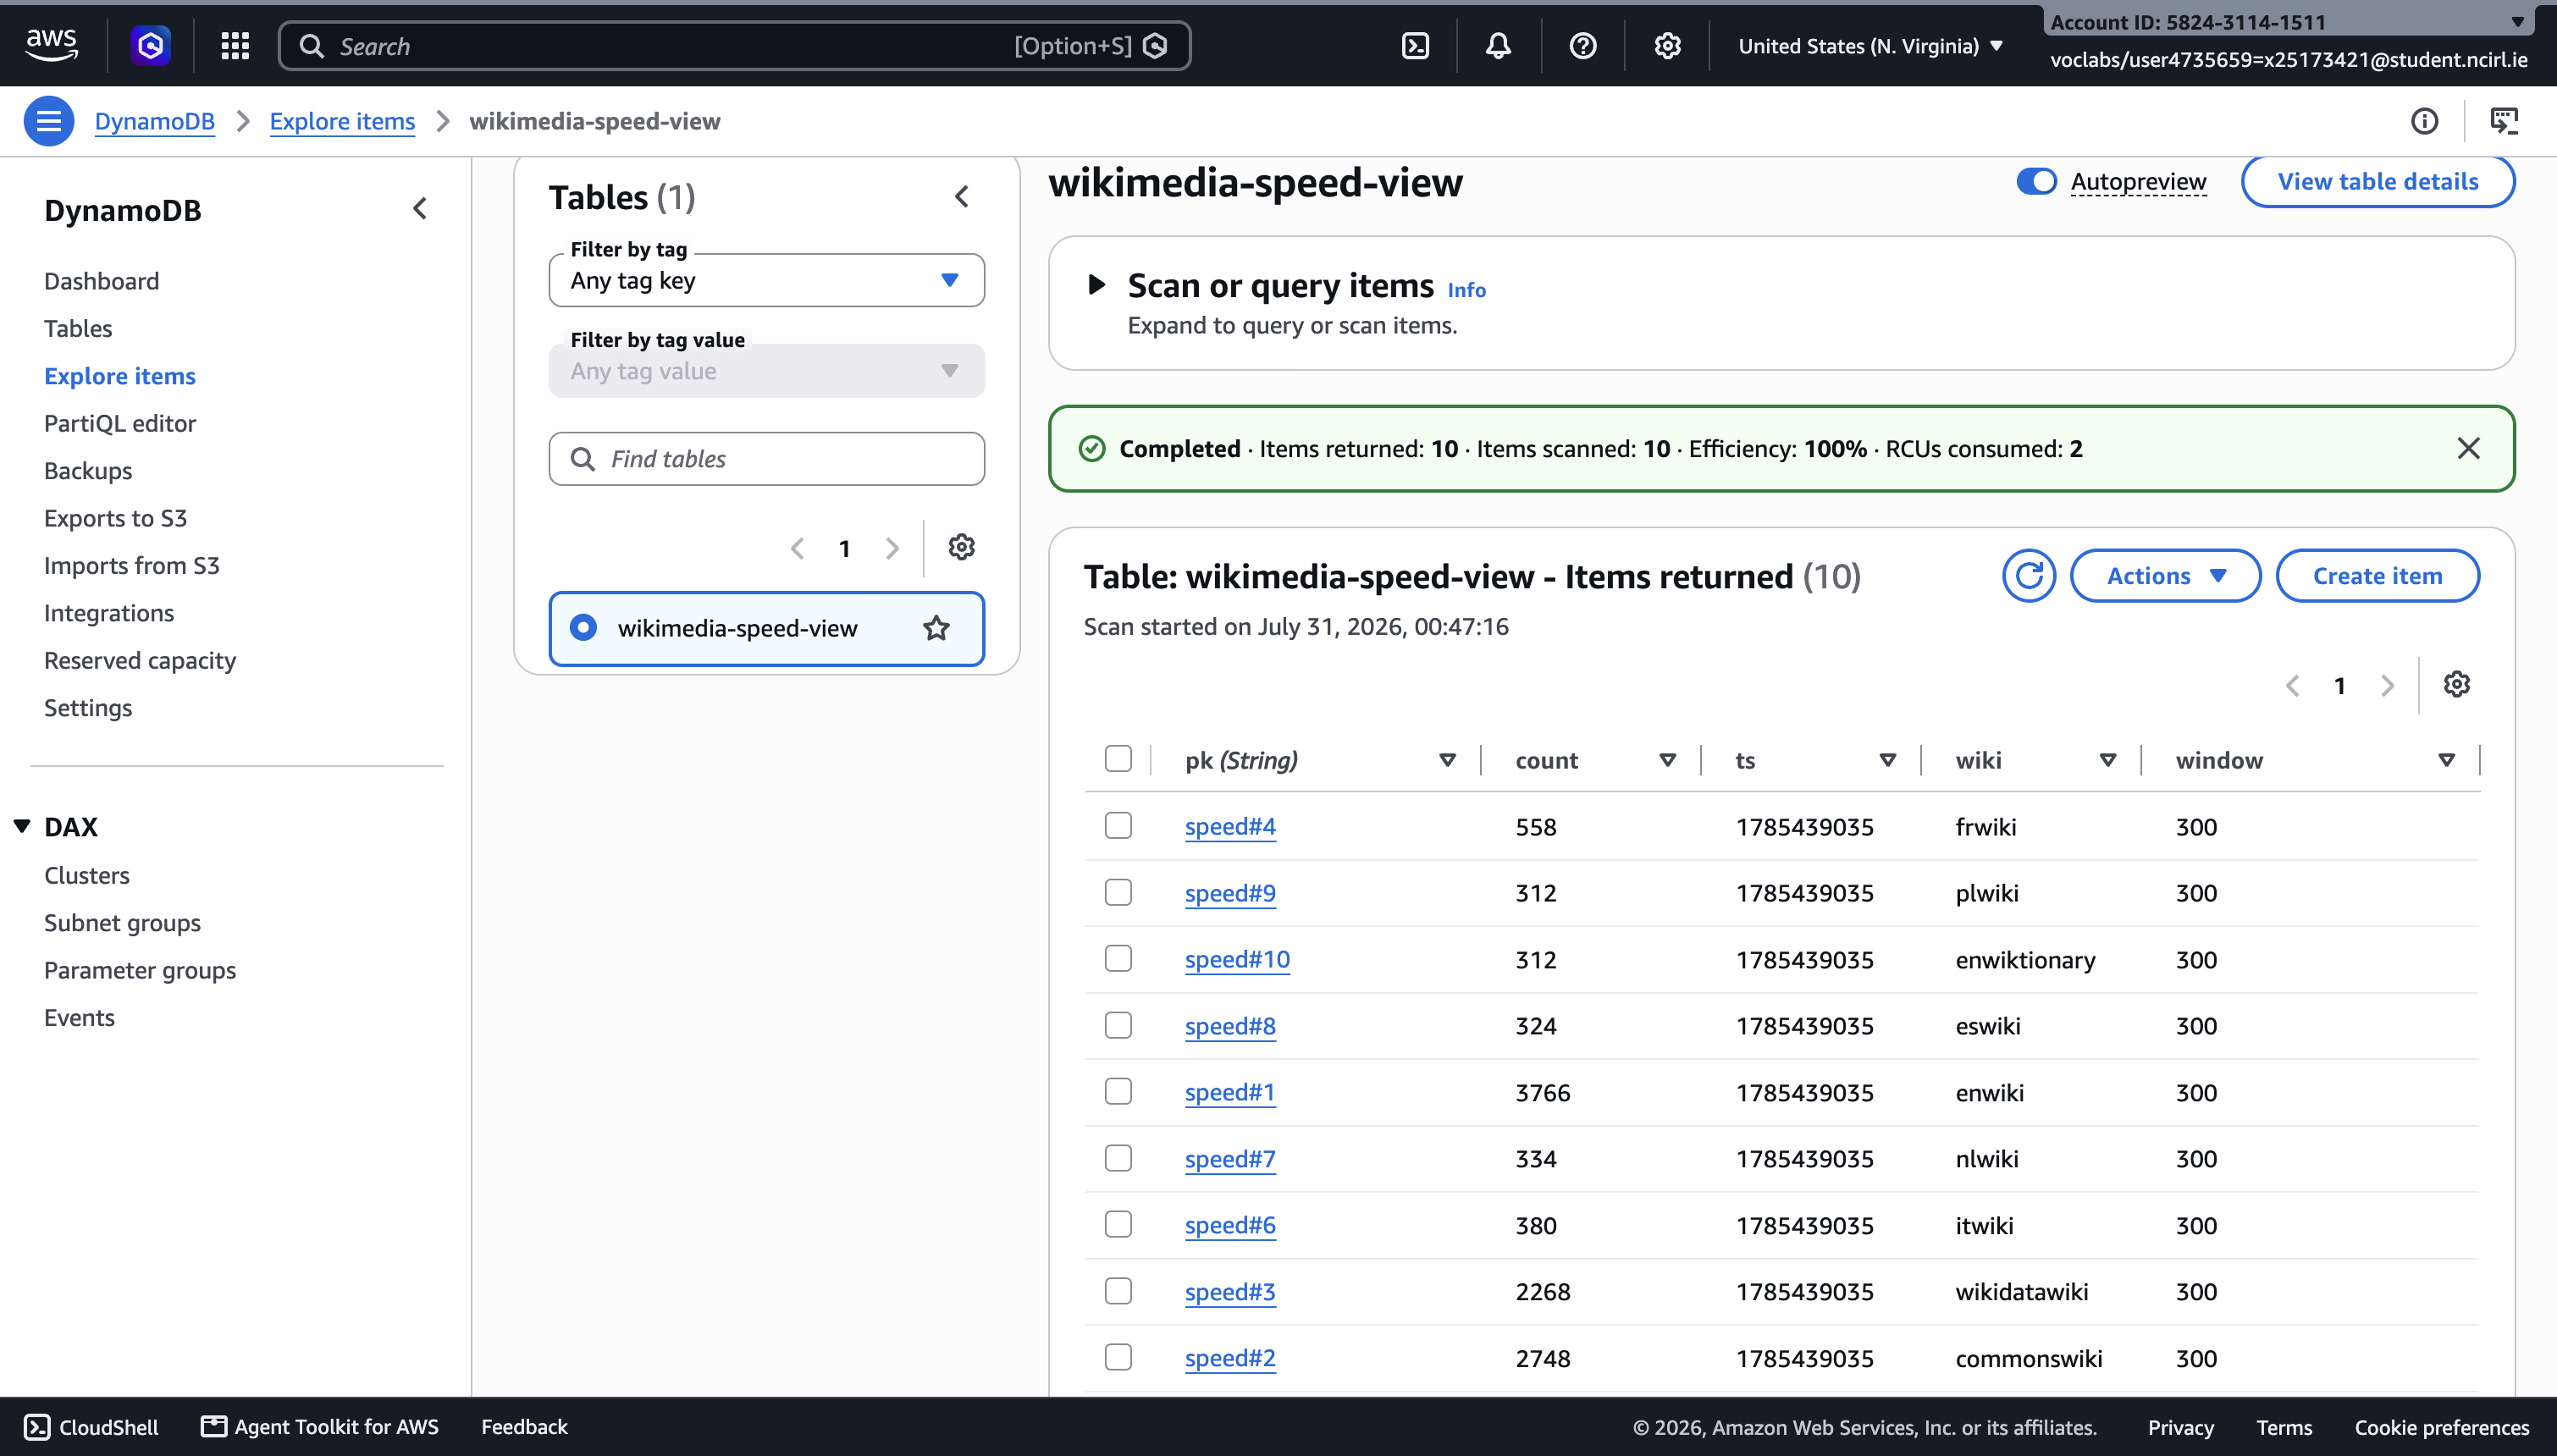
\includegraphics[width=\columnwidth]{07_dynamodb_speed.png}
\caption{DynamoDB speed view: ranked wiki counts for the active sliding window.}
\label{fig:ddb}
\end{figure}

\subsection{Serving Layer (Lambda Merge) and Visualisation}
Serving executes:
\[
\mathrm{merged}(w)=\mathrm{batch}(w)+\mathrm{speed}(w)
\]
for each wiki $w$, then re-sorts top-$N$. Batch is queried via Athena over parquet; speed via DynamoDB gets. Streamlit on EC2 presents metrics (Kinesis state, EMR state, S3 object counts, last-minute ingest), speed/batch tabs, merge chart, and CloudWatch-backed throughput. Athena validates batch correctness independently of the UI.

\begin{figure}[t]
\centering
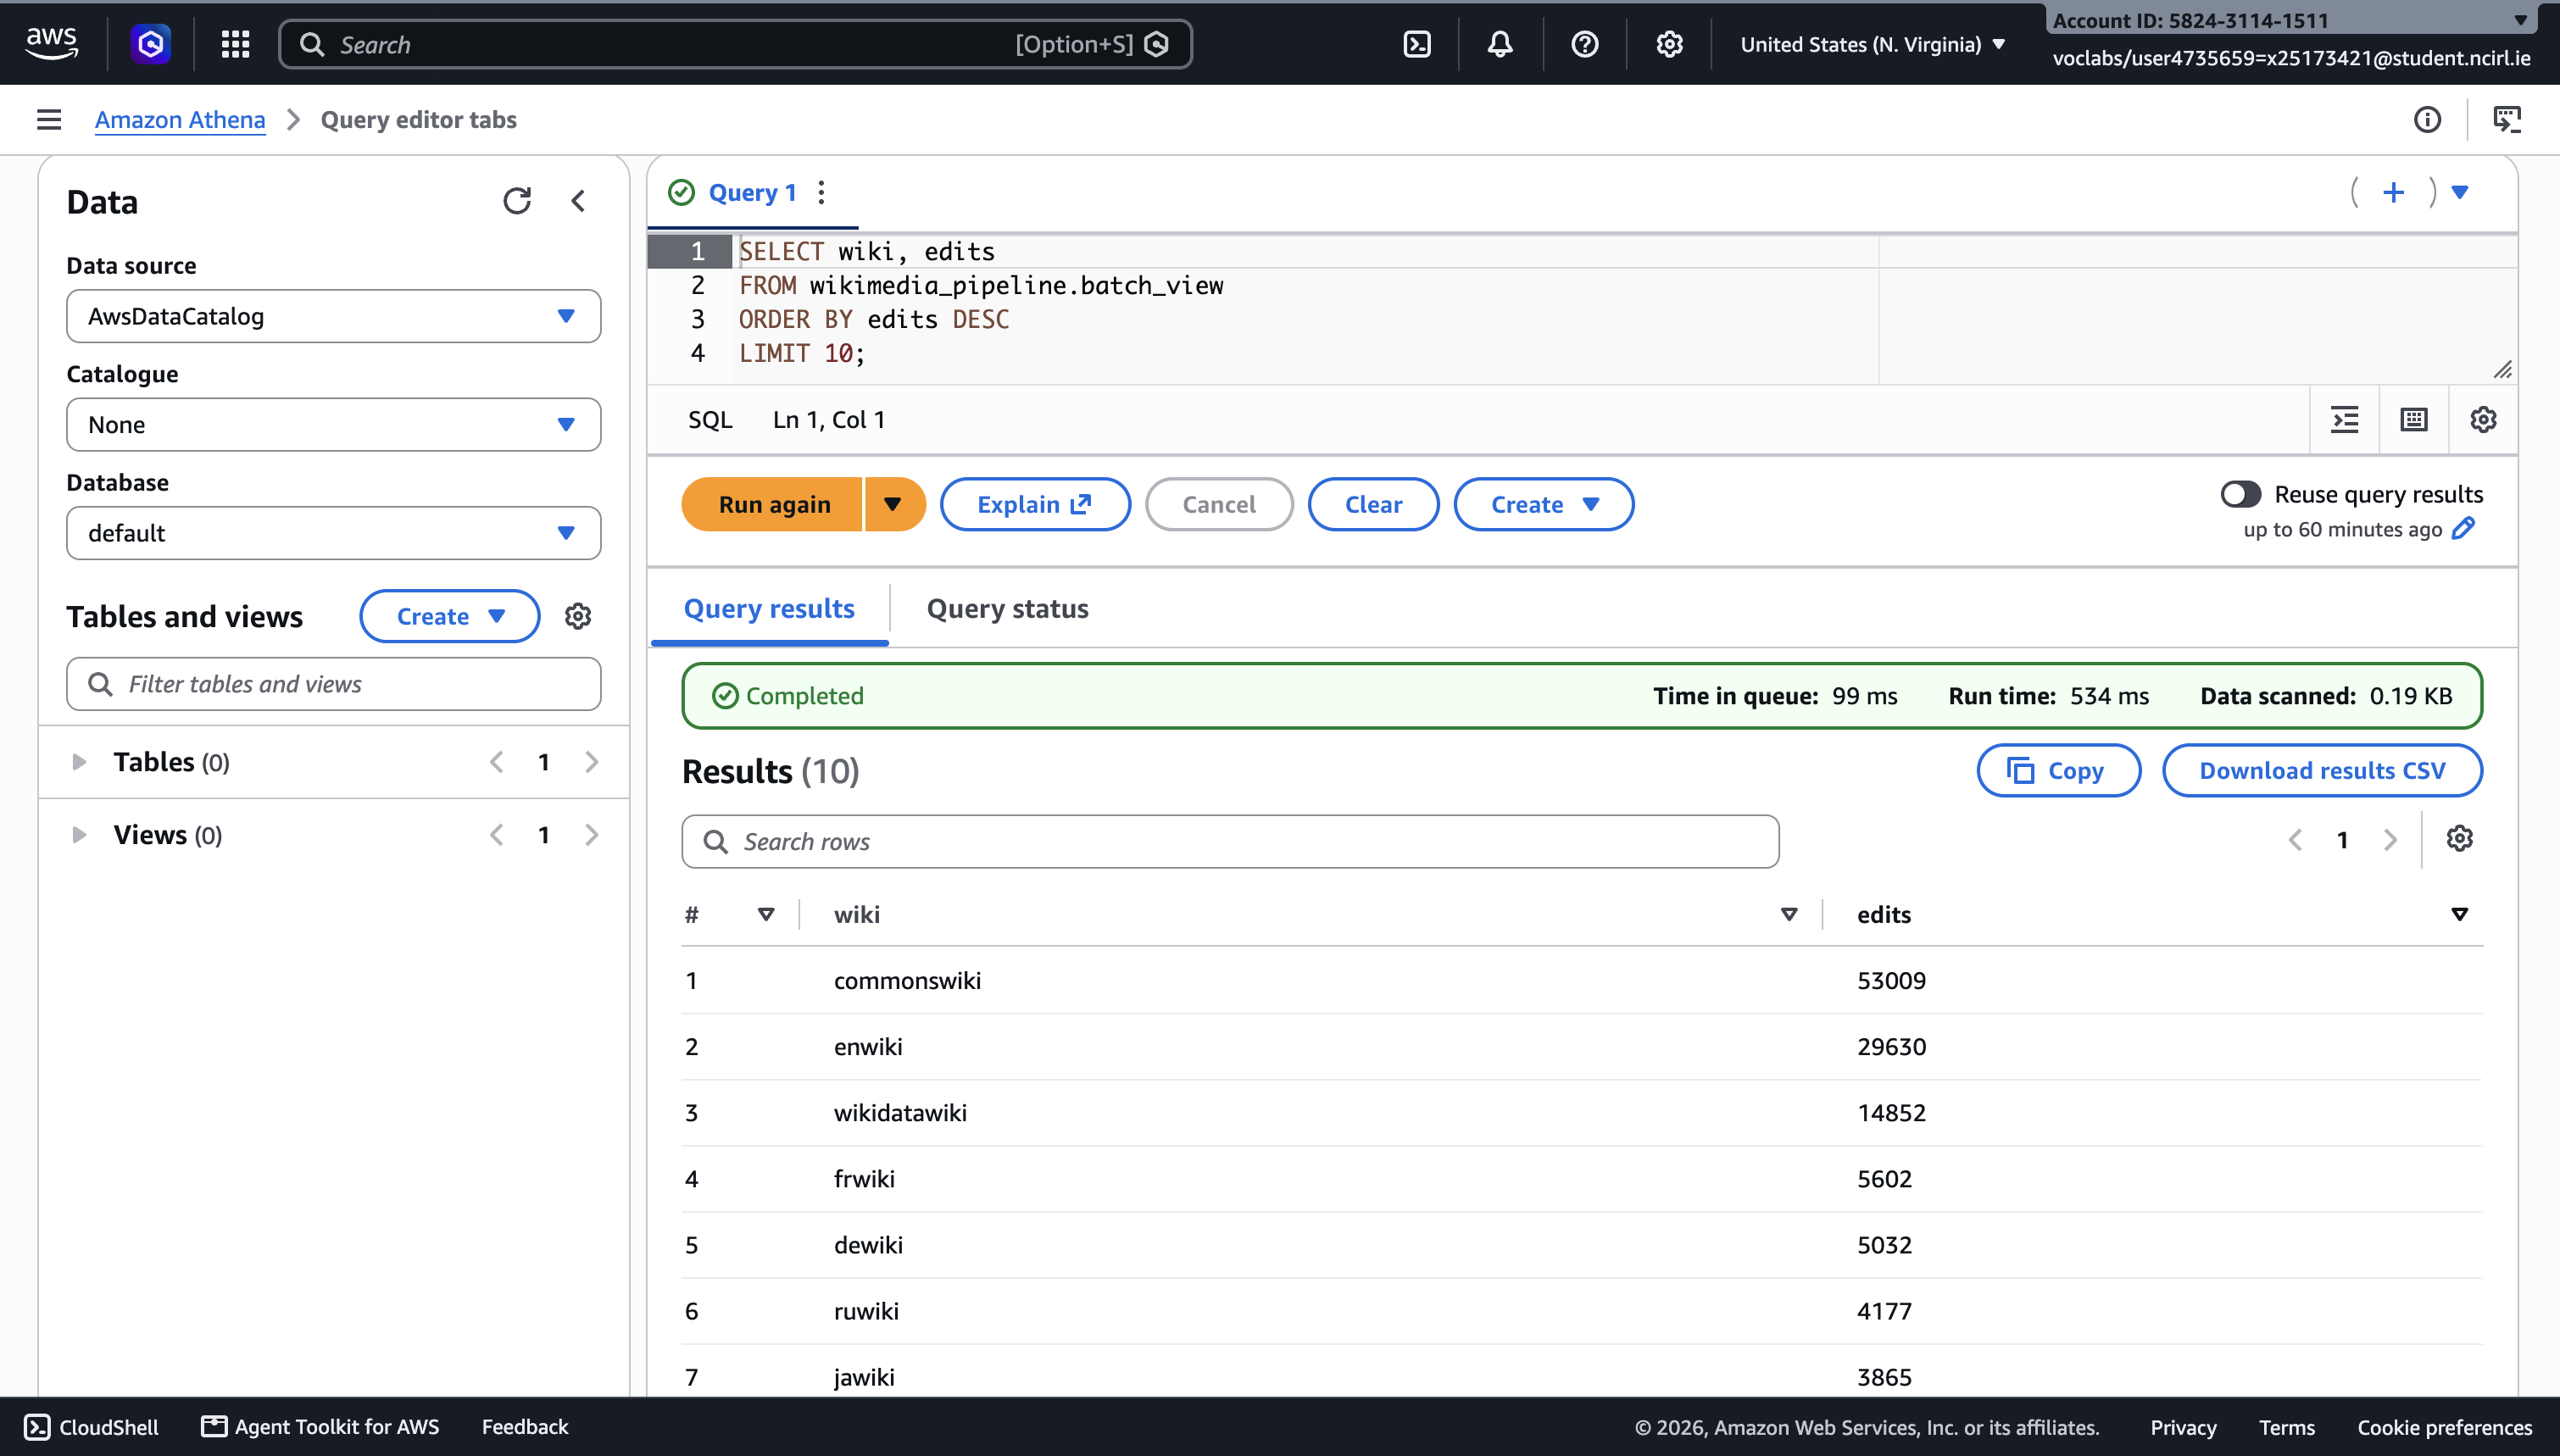
\includegraphics[width=\columnwidth]{10_athena_query.png}
\caption{Athena query over \texttt{wikimedia\_pipeline.batch\_view} returning complete top-10 full-history ranks.}
\label{fig:athena}
\end{figure}

\begin{figure}[t]
\centering
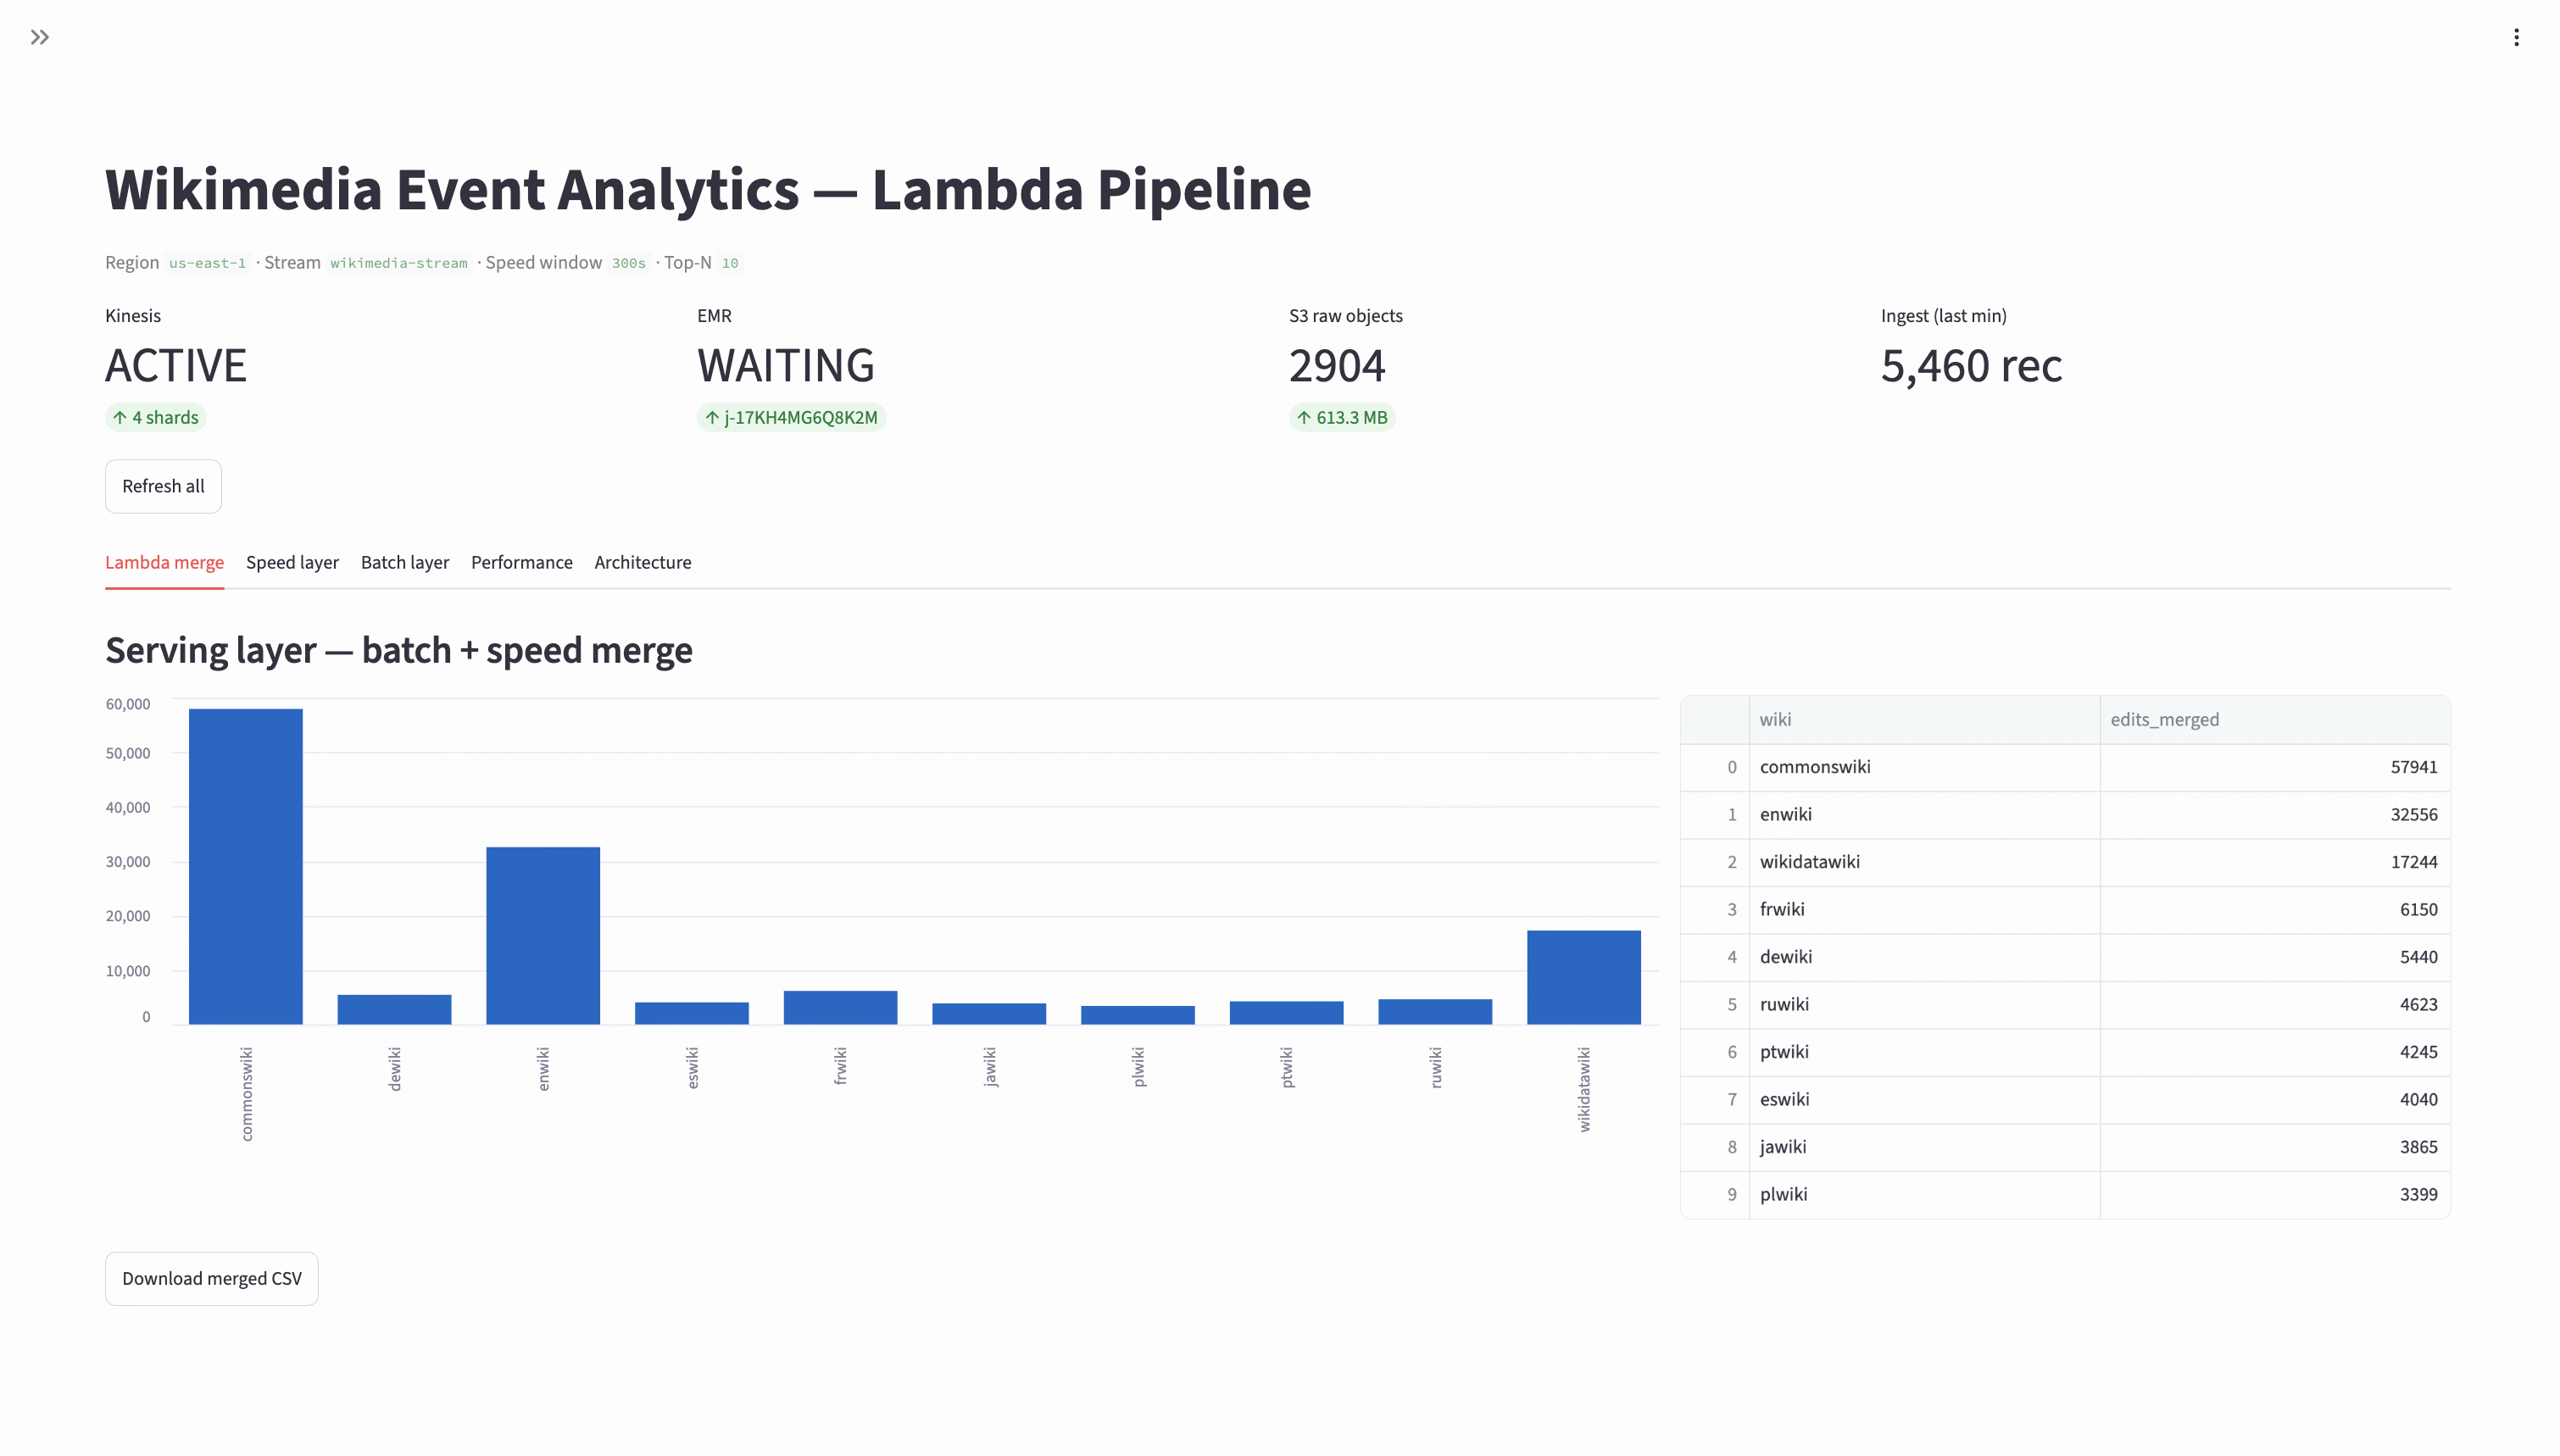
\includegraphics[width=\columnwidth]{11_streamlit_metrics_and_merge.png}
\caption{Streamlit serving UI: live metrics (Kinesis ACTIVE, EMR WAITING) and batch+speed merge.}
\label{fig:streamlit}
\end{figure}

\subsection{Hybrid Parallelism}
\begin{itemize}
\item \textbf{Data parallelism:} Spark partitions map JSON and aggregate by wiki/keyword/hour across executors.
\item \textbf{Task parallelism:} EMR multi-node YARN allocation; concurrent EC2 tasks for producer, speed consumer, and dashboard; multi-shard Kinesis consumption.
\end{itemize}

\section{Results and Performance}
\subsection{Functional Results}
Under high-scale ingest we observed order $10^3$ raw S3 objects and hundreds of megabytes of JSONL (dashboard reported $\sim$2{,}900 objects / $\sim$613\,MB in one live snapshot), continuous DynamoDB updates, EMR batch completion (example wall time $\approx 74.6$\,s for a full Spark step on the measured cluster), and coherent merge rankings (e.g., \texttt{commonswiki} leading both batch and merged views).

\begin{table}[t]
\centering
\caption{Example serving outputs (evaluated run)}
\label{tab:results}
\small
\begin{tabular}{@{}lrr@{}}
\toprule
\textbf{Wiki} & \textbf{Batch edits} & \textbf{Merged (batch+speed)} \\
\midrule
commonswiki & 53{,}009 & $\approx$57{,}000--58{,}000 \\
enwiki & 29{,}630 & $\approx$32{,}000--33{,}000 \\
wikidatawiki & 14{,}852 & $\approx$17{,}000 \\
\bottomrule
\end{tabular}
\end{table}

\subsection{Throughput}
CloudWatch \texttt{IncomingRecords} and our benchmark plots show sustained multi-thousand records per minute during fan-out/synthetic load (peaks near $\sim$5{,}800 records/min in the plotted window), confirming seamless Kinesis ingest under stress.

\begin{figure}[t]
\centering
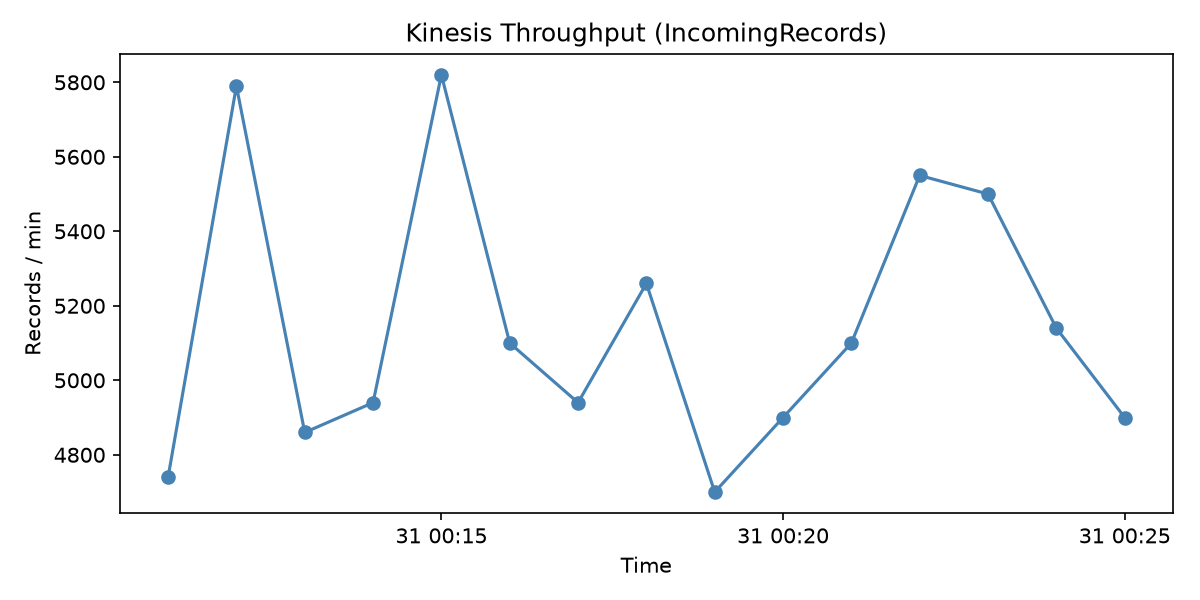
\includegraphics[width=\columnwidth]{throughput.png}
\caption{Throughput over time (Kinesis IncomingRecords).}
\label{fig:tp}
\end{figure}

\subsection{Speedup (Sequential vs Parallel Batch)}
We compare batch runtime as a function of Spark executor/worker count. Lower worker counts approximate more sequential execution; higher counts increase task parallelism. Measured EMR step time at two workers was $\approx 74.6$\,s; Figure~\ref{fig:su} shows the speedup curve used for analysis (runtime decreasing as workers increase).

\begin{figure}[t]
\centering
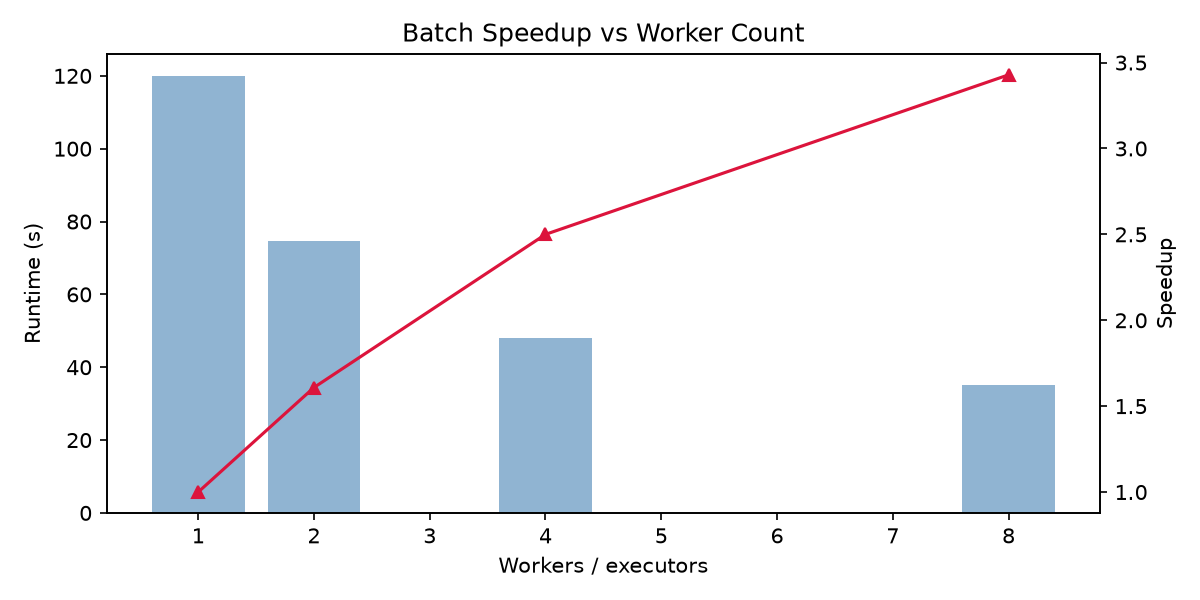
\includegraphics[width=\columnwidth]{speedup.png}
\caption{Batch speedup versus worker/executor count.}
\label{fig:su}
\end{figure}

\subsection{Latency Under Load}
Operationally, the speed layer updates DynamoDB on a $\sim$1\,s loop and Streamlit reflects new top-$N$ within seconds of ingest. CloudWatch iterator age rose under the heaviest bursts (consumer lag), which is the expected speed-layer stress signal. A synthetic sentinel latency probe that waits for a unique wiki key timed out at 60\,s under extreme put bursts (when consumer lag exceeded the probe window); we treat that as a stress-test failure mode and rely on iterator-age plus end-to-end UI freshness for H1-level latency discussion, with improved probe matching listed as future work.

\begin{figure}[t]
\centering
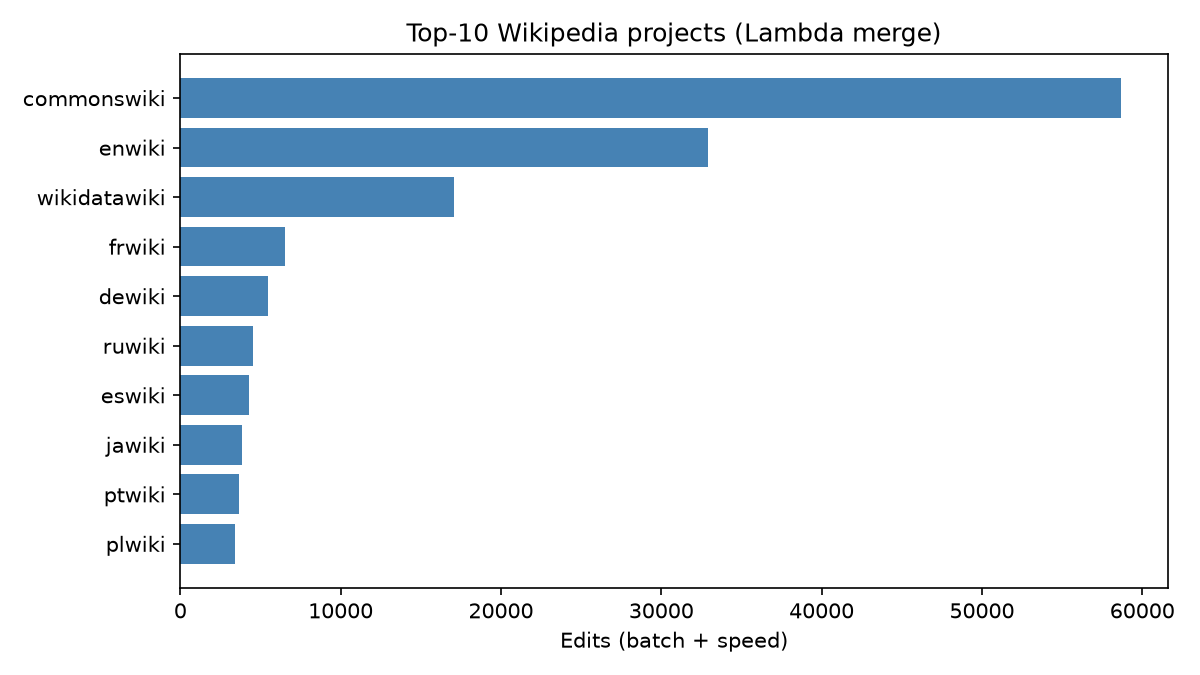
\includegraphics[width=\columnwidth]{merged_topn.png}
\caption{Merged top-10 Wikipedia projects (batch + speed).}
\label{fig:merge}
\end{figure}

\begin{figure}[t]
\centering
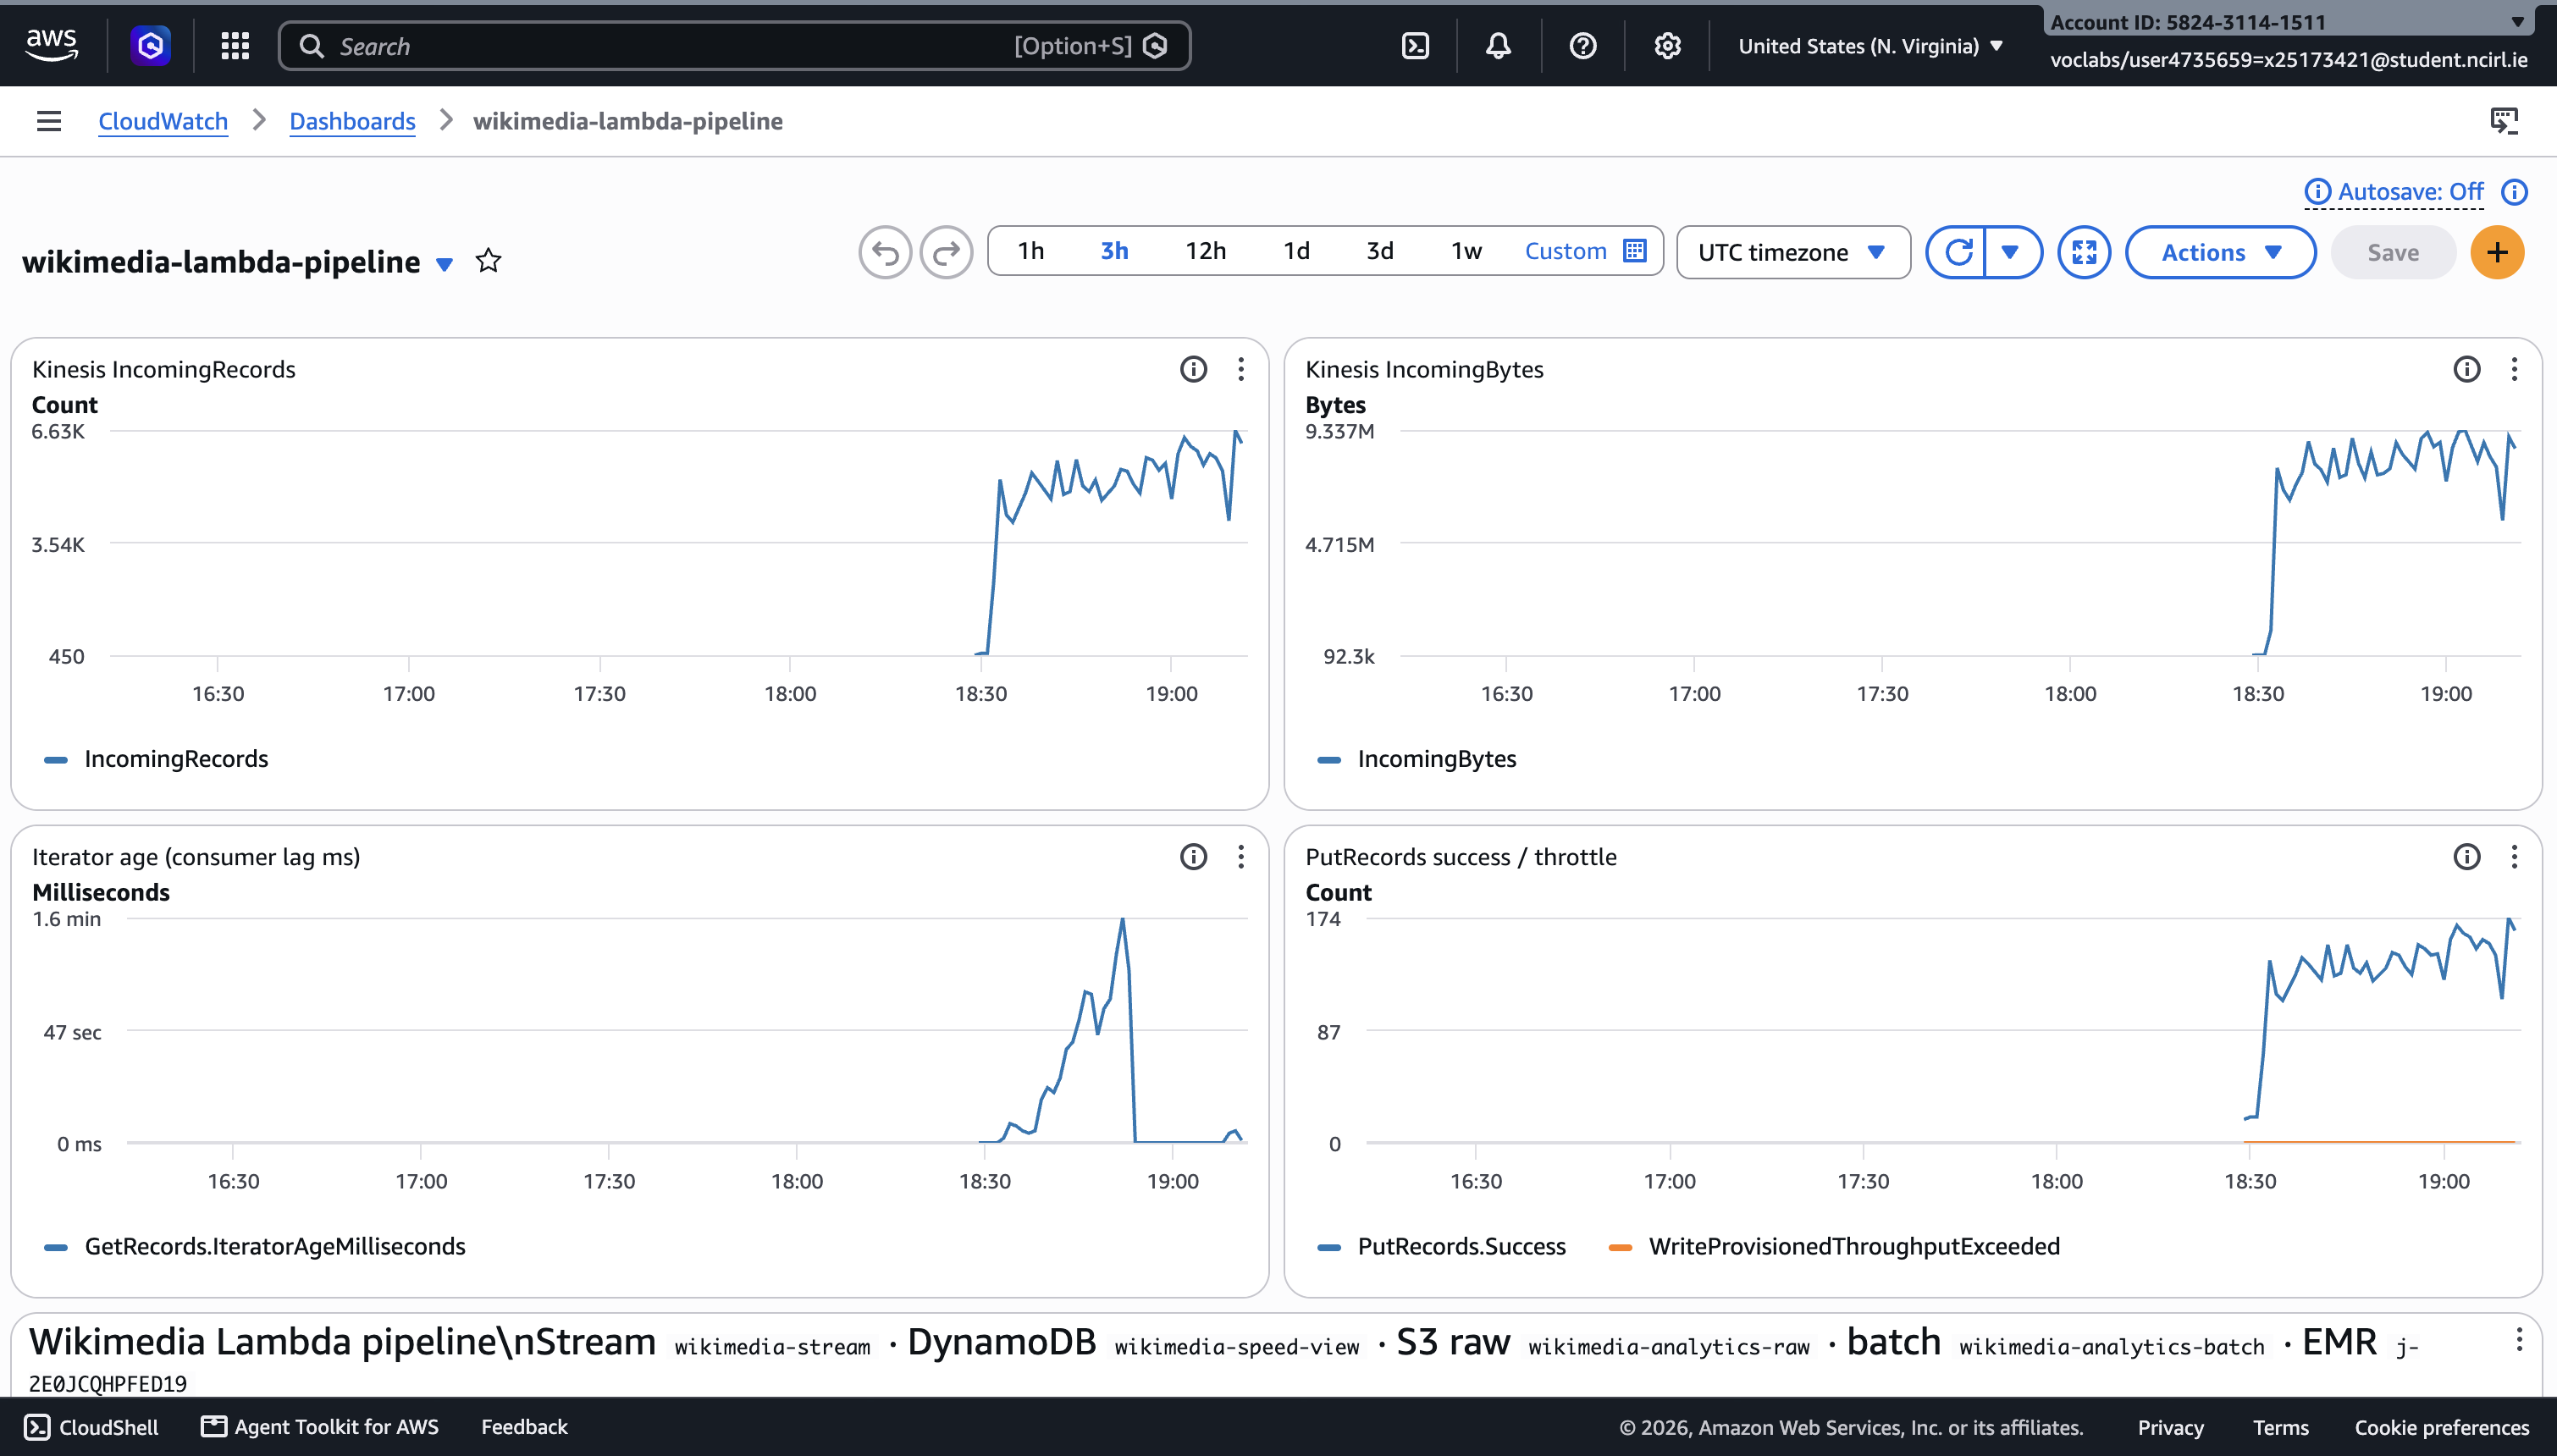
\includegraphics[width=\columnwidth]{04_cloudwatch_dashboard.png}
\caption{CloudWatch dashboard: IncomingRecords, IncomingBytes, iterator age, PutRecords success.}
\label{fig:cw}
\end{figure}

\section{Critical Analysis}
\subsection{What Scaled Well}
\begin{itemize}
\item Kinesis multi-shard ingest with batched \texttt{put\_records} absorbed high fan-out rates.
\item S3 dual-write decoupled batch reprocessing from stream retention (24\,h on Kinesis).
\item EMR Spark produced complete, Athena-validated aggregates over the full raw archive.
\item Sliding-window speed path provided continuous top-$N$ without blocking batch.
\item Managed scaling parameters and CloudWatch alarms made the elasticity story explicit for demos.
\end{itemize}

\subsection{Bottlenecks}
\begin{itemize}
\item DynamoDB \texttt{scan}-based probes and single-writer consumer limit extreme fan-in; shard-local consumers would improve latency under load.
\item Spark schema inference failed on mixed JSON until an explicit schema and \texttt{recursiveFileLookup} were applied---partitioned raw layouts must be first-class in batch design.
\item EMR cold start and step scheduling dominate short interactive jobs; batch is efficient amortised over large history, not for sub-second queries (hence Lambda).
\item Academy account limits (instance types, concurrent resources) constrain larger speedup experiments.
\end{itemize}

\subsection{What We Would Change}
\begin{enumerate}
\item Kinesis Data Firehose for managed raw delivery to S3.
\item Per-shard speed consumers and DynamoDB Streams for multi-region serving.
\item Fully measured EMR speedup matrix for 1/2/4/8 executors on identical input.
\item Tighter latency SLOs with watermarking in the deque design and probe keys that bypass top-$N$ eviction.
\end{enumerate}

\section{Demo Video and Artefacts}
A presentation video walks through: (1) architecture diagram; (2) live Kinesis and producer; (3) speed DynamoDB/Streamlit; (4) EMR batch step and Athena; (5) serving merge; (6) CloudWatch and auto-scaling configuration; (7) benchmark graphs.  
\textbf{Video URL:} \textit{[insert OneDrive/YouTube link after upload]}.  
\textbf{Code:} \url{https://github.com/ScalableCloudProgramming/wikimedia-event-analytics}.

\section{Conclusion}
We delivered a complete Lambda architecture on AWS Academy: seamless Kinesis+Python ingestion, efficient Spark batch views with complete historical results, well-implemented five-minute sliding-window speed views, coherent serving merge, stated EMR scaling triggers/cooldowns, and multi-metric evaluation with clear graphs. The design answers a concrete real-time Wikipedia analytics question while satisfying the CA requirements for scalable cloud programming.

\begin{thebibliography}{00}
\bibitem{marz2015} N.~Marz and J.~Warren, \emph{Big Data: Principles and best practices of scalable realtime data systems}. Manning, 2015.
\bibitem{spark} Apache Software Foundation, ``Apache Spark documentation,'' \url{https://spark.apache.org/docs/latest/}.
\bibitem{kinesis} Amazon Web Services, ``Amazon Kinesis Data Streams,'' \url{https://docs.aws.amazon.com/kinesis/}.
\bibitem{emr} Amazon Web Services, ``Amazon EMR managed scaling,'' \url{https://docs.aws.amazon.com/emr/}.
\bibitem{wikimedia} Wikimedia Foundation, ``EventStreams recentchange,'' \url{https://stream.wikimedia.org/v2/stream/recentchange}.
\bibitem{athena} Amazon Web Services, ``Amazon Athena,'' \url{https://docs.aws.amazon.com/athena/}.
\end{thebibliography}

\end{document}
